\section{Introduction}

The scientific community is currently experiencing a surge in interest in techniques that offer higher spatial resolution, a trend intrinsically linked to advancements in technology. Since the pioneering contributions of \citet{Egli2000}, implementing high-resolution scanning magnetic microscopy (SMM) methodologies has become increasingly feasible in paleomagnetic research, offering an alternative to conventional approaches that typically analyze entire rock samples. This method facilitates the discernment of magnetization heterogeneities undetectable at larger scales. Nonetheless, these SMM techniques require data processing to unravel the information contained in the potential field measured. Dealing with potential fields, in general, could be very challenging due to the ambiguity associated with the data itself, generating non-unique results during the inversion \citep{Blakely1996}. A common way to circumvent the non-uniqueness is integrating prior knowledge about the sources causing the anomaly, such as the position of a known magnetized source \citep{Fabian2019}. The X-ray computed tomography (microCT) technique is a good example of the application of the additional information \citep[\textit{e.g.}][]{DeGroot2018, DeGroot2021, Koster2023}, which can be further refined by the inversion of the magnetic moment using spherical harmonic \citep[\textit{e.g.}][]{CortesOrtuno2021, CortesOrtuno2022}.

Another way to insert additional information without the requirement of performing new measurements was proposed by \citet{Souza-Junior2023b}, which uses techniques extrapolated from aeromagnetic surveys, such as the Euler deconvolution, due to its similarity with the SMM \citep{Weiss2007}. The methodology is designed for the semi-automatic estimation of position and dipole moments for individual grains and consists of three main steps. First, it combines classic potential field data processing (like total gradient amplitude) with image processing techniques (such as histogram stretching, and edge detection) to identify and isolate the magnetic fields of individual sources into data windows. Next, the 3D position of the source is estimated through the Euler deconvolution equation based on the magnetic microscopy field measurements within each data window. Finally, the 3-component dipole moment vector is obtained using a least-square estimator assuming that a dipolar source causes the magnetic anomaly. The methodology was originally designed for computational efficiency and stability. However, it infringes on the mathematical premise of inversion theory states that the sampled area must be encapsulated by inversion domain \citep{Baratchart2013, Lima2013} thus, more often than not, failing to account for the mutual interference between sources and/or shifts in the measured field. This study introduces a novel approach that aims to account for the mutual interference of the sources in the methodology proposed by \citet{Souza-Junior2023b}, as well as any shift in the field. Through refining the window-based approach, the proposed methodology presents a significant advancement in magnetic microscopy, with potential application for paleomagnetic studies. 


%%%%%%%%%%%%%%%%%%%%%%%%%%%%%%%%%%%%%%%%%%%%%%%%%%%%%%%%%%%%%%%%%%%%%%%%%%%%%%%
\section{Methodology}

To fully leverage the advancement of magnetic microscopy for paleomagnetic studies, we must isolate the individual contribution of the stable remnant magnetization carriers within the rock fabric. This is also related to a major limitation of the inversion procedures used to retrieve the information carried by these grains. To guarantee the solution's uniqueness, prior information about the sources must be provided. The novelty of Euler deconvolution application to magnetic microscopy data, developed by \citet{Souza-Junior2024}, showed the possibility of individual estimation of magnetic grains without additional measurements. However, the technique violates the principles of inverse theory by ignoring non-encapsulated effects within the inversion domain, \textit{i.e.} mutual influence of sources. This study explores a new methodology to effectively manage interfering sources during the inversion process, which is designed to mitigate the magnetic sources' interference and enhance the precision of the inversion analyses proposed.


\subsection{Magnetic vector inversion with interfering sources}\label{inversion-section}

The interference source methodology is proposed to enhance the accuracy of window-based inversion analyses in magnetic data, particularly in scenarios where stronger magnetic fields could introduce distortions in the results. Since an edge detection algorithm is applied to the total gradient anomaly map to segment the data windows of the magnetic sources, which follow the descending order of blob magnitude. This is directly proportional to the magnetic signal of the sources. Hence, it can be used to account for the effect of stronger sources. This process is divided into distinct steps from locating the position of the magnetic carriers to the estimation of their magnetic moment.


\subsubsection{Position estimation}
    Euler deconvolution (ED) is widely applied in aeromagnetic surveys \citep{Barbosa2011, Melo2013, Melo2018} to obtain a 3D position estimation \cite[after][]{Reid1990}. The only assumption is the source's shape given by the structural index ($\eta$), in the case of a dipole $\eta = 3$. The Euler's homogeneity equation is then given by
    
        \begin{equation}
        \label{eq_euler_homogeneity}
        (x - x_c)\partial_x f
        + (y - y_c)\partial_y f
        + (z - z_c)\partial_z f
        = (b - f)\eta
        \ .
        \end{equation}
    
    \noindent{The solution of the ED is performed in the rearranged pseudo-parametric model}
    
    \begin{equation}
    x_c \partial_x f + y_c \partial_y f + z_c \partial_z f + \eta b
    =
    x \partial_x f + y \partial_y f + z \partial_z f + \eta f
    \ .
    \end{equation}
    
    For a given magnetic field anomaly ($f$) and its directional derivatives ($\partial \alpha f$, $\alpha = x, y, z$ ) at the i\textsuperscript{th} observation point ($x_i, y_i, z_i$), $i=1, 2,..., N$, we can describe a $N \times 4$ system of equations as:
    
    \begin{equation}
    {\overbrace{
    \begin{bmatrix}
      {\partial_x f}_1 & {\partial_y f}_1 & {\partial_z f}_1 & \eta \\
      {\partial_x f}_2 & {\partial_y f}_2 & {\partial_z f}_2 & \eta \\
      \vdots & \vdots & \vdots & \vdots \\
      {\partial_x f}_N & {\partial_y f}_N & {\partial_z f}_N & \eta
    \end{bmatrix}
    }^{\mathbf{G}}}_{N \times 4}
    {\overbrace{
    \begin{bmatrix}
      x_c \\ y_c \\ z_c \\ b
    \end{bmatrix}
    }^{\mathbf{p}}}_{4 \times 1}
    =
    {\overbrace{
    \begin{bmatrix}
      x_1 {\partial_x f}_1 + y_1 {\partial_y f}_1 + z_1 {\partial_z f}_1 + \eta f_1 \\
      x_2 {\partial_x f}_2 + y_2 {\partial_y f}_2 + z_2 {\partial_z f}_2 + \eta f_2 \\
      \vdots \\
      x_N {\partial_x f}_N + y_N {\partial_y f}_N + z_N {\partial_z f}_N + \eta f_N \\
    \end{bmatrix}
    }^{\mathbf{h}}}_{N \times 1}
    \ .
    \end{equation}
    
    The solution of this linear system is defined by the vector $\mathbf{p}$ that minimizes the misfit function, $\phi(\mathbf{p})$, given by the sum of the squared differences between the pseudo-observation data ($\mathbf{h}^o$) and the predicted data ($\mathbf{h}$):
    
    \begin{equation}
    \label{function_phi}
    \phi(\mathbf{p}) = \min_{\mathbf{p}} \| \mathbf{G}\mathbf{p} - \mathbf{\mathbf{h}^o} \|_2^2\ = \min_{\mathbf{p}} \| \mathbf{h} - \mathbf{\mathbf{h}^o} \|_2^2\
    .
    \end{equation}
    
    \noindent{Which is obtained by applying}
    
    \begin{equation}
    \label{euler_solution}
    \mathbf{p} = {[\mathbf{G}^T \mathbf{G}]}^{-1} [\mathbf{G}^T \mathbf{h}^o]\ .
    \end{equation}
    
    The parameters vector $\mathbf{p}$ contains the dipolar source's coordinates, $x_c$, $y_c$, and $z_c$. It also contains the base level ($b$), the background field within the window.
    
\subsubsection{Magnetic moment inversion} 
    One of the main drawbacks of estimating a physical property from potential data, such as the dipole moment vector $(m_x, m_y, m_z)$, lies in its ambiguity \citep{Blakely1996}. This is commonly circumvented by adding additional information about the sources (\textit{e.g.} shape, position, and size). Therefore, the ED solution (Equation~\ref{euler_solution}) might be used as prior information to recover the dipole moment of the sources causing the anomaly within the window data.
    
     Following \citet{Oliveira2015Estimation}, the vertical component of the magnetic field ($fz$), measured at the i\textsuperscript{th} observation point ($i=1, 2, ..., N$), produced by a dipolar source located in the Cartesian coordinates $x_c, y_c$ and $z_c$, can be calculated using:

     \begin{equation}
    \label{eq_dipole_bz}
    {\overbrace{\begin{bmatrix}
    \dfrac{\mu_0}{4\pi} \dfrac{\partial^2}{\partial z \partial x} \dfrac{1}{r_i}
    & \dfrac{\mu_0}{4\pi} \dfrac{\partial^2}{\partial z \partial y} \dfrac{1}{r_i}
    & \dfrac{\mu_0}{4\pi} \dfrac{\partial^2}{\partial z \partial z} \dfrac{1}{r_i}
    \end{bmatrix}}^{\mathbf{A}}}_{N \times 3}
    {\overbrace{{\begin{bmatrix}
    m_x \\ m_y \\ m_z
    \end{bmatrix}}}^{\mathbf{m}}}_{3 \times 1}
    =
    ~{\overbrace{\begin{bmatrix}
    fz_i
    \end{bmatrix}}^{\mathbf{d}}}_{N \times 1}
    \ .
    \end{equation}

    \noindent{
    Where $r = \sqrt{(x_i - x_c)^2 + (y_i - y_c)^2 + (z_i - z_c)^2}$ is the distance between the observation point $(x_i, y_i, z_i)$ and the dipolar source $(x_c, y_c, z_c)$, $\mu_0$ is the vacuum magnetic permeability, and the second-order derivative terms in Equation~\ref{eq_dipole_bz} are:
    
    \begin{equation}
    \begin{aligned}
    \dfrac{\partial^2}{\partial z \partial x} \dfrac{1}{r_i} &=
    \dfrac{3(z_i - z_c)(x_i - x_c)}{{r_i}^5}\ ,
    \\
    \dfrac{\partial^2}{\partial z \partial y} \dfrac{1}{r_i} &=
    \dfrac{3(z_i - z_c)(y_i - y_c)}{{r_i}^5}\ ,
    \\
    \dfrac{\partial^2}{\partial z \partial z} \dfrac{1}{r_i} &=
    \dfrac{3(z_i - z_c)^2}{{r_i}^5} - \dfrac{1}{{r_i}^3}\ .
    \end{aligned}
    \end{equation}}

    The $N \times 3$ linear system in the Equation~\ref{eq_dipole_bz} has its solution defined by the parameter vector ($\mathbf{m}$) that minimizes the misfit function $\psi(\mathbf{m})$ given by the residual between the predicted ($\mathbf{\mathbf{d}}$) and observed ($\mathbf{\mathbf{d}^o}$) data vectors. The latter is also corrected by the background field ($b$) obtained with the ED. Then the misfit function $\psi(\mathbf{m})$ can be written as:
   
    \begin{equation}
    \label{psi_function}
    \psi(\mathbf{m}) = \min_{\mathbf{m}} \| \mathbf{A}\mathbf{m} - \mathbf{\mathbf{d}^o} \|_2^2\ = \min_{\mathbf{m}} \| \mathbf{d} - (\mathbf{\mathbf{d}^o}-b) \|_2^2\
    .
    \end{equation}

    The parameters vector ($\mathbf{m}$), containing the Cartesian components of the magnetic moment, can be obtained by the least-squares estimator:

    \begin{equation}
    \label{dipole_moment_solution}
    \mathbf{m} = {[\mathbf{A}^T \mathbf{A}]}^{-1} [\mathbf{A}^T (\mathbf{d}^o - b)]\ .
    \end{equation}
        
\subsubsection{Simplex optimization} 
     The forward model of the dipole's vertical component anomaly from the Equation~\ref{eq_dipole_bz} can be rewritten as:

    \begin{equation}
        \small
        \label{bz_dipole_equation}
        {d}_{i} = \frac{\mu_0}{4 \pi} \left [ 3 \frac{ (z_i-z_c) \left ( m_x (x_i-x_c) + m_y (y_i-y_c) + m_z (z_i-z_c) \right )}{{r_i}^5} - \frac{m_z}{{r_i}^3} \right ] .
    \end{equation}
    
     After obtaining the initial estimates of the 3D position $(x_{c0}, y_{c0}, z_{c0})$ and the dipole moment vector $(m_{x0}, m_{y0}, m_{z0})$, both position and magnetic moment might still be refined to improve the model results. For this process, the optimization technique utilized was the Scipy Nelder-Mead method \citep{2020SciPy-NMeth}, which employs these six parameters obtained in previous steps as initial guesses for the goal function (Equation~\ref{bz_dipole_equation}). The misfit function to be minimized is given by:
    
    \begin{equation}
    \label{misfit_equation}
    \xi (x_c, y_z, z_c, m_x, m_y, m_z) = \| (\mathbf{d}^{o}-b) - \mathbf{d} \|^2.
    \end{equation} 
    
     The Nelder-Mead method, a gradient-free optimization technique, systematically searches the optimal solution of Equation~\ref{misfit_equation} by iteratively adjusting a simplex in the parameter space \citep{Nelder-Mead1965}. This is particularly useful for optimizing functions where gradients are difficult to compute or unavailable. 
     
     However, the substantial difference of up to seven orders of magnitude between the position and the magnetic moment poses a challenge. This dissimilarity directly affects the simplex operations and has been addressed by normalizing the initial magnetic moment magnitude ($m_0 = \sqrt{{m_{x0}}^2+{m_{y0}}^2+{m_{z0}}^2}$), as follows:
     \begin{align}
    \label{normalizing_m_parameters}
    {m_x}^{j+1} &= \frac{{m_x}^{j}}{m_0}, & {m_y}^{j+1} &= \frac{{m_y}^{j}}{m_0}, & \text{and} & &{m_z}^{j+1} &= \frac{{m_z}^{j}}{m_0}
    \ .
    \end{align}
     
\noindent{Which was also applied for the position vector using the initial position estimates:}
     \begin{align}
    \label{normalizing_h_parameters}
    {x_c}^{j+1} &= \frac{{x_c}^{j}}{x_{c0}}, & {y_c}^{j+1} &= \frac{{y_c}^{j}}{y_{c0}}, & \text{and} & &{z_c}^{j+1} &= \frac{{z_c}^{j}}{z_{c0}}
    \ .
    \end{align}
    
% \begin{align}
% \label{normalizing_parameters}
% {x_c}^{j+1} &= \frac{{x_c}^{j}}{x_{c0}}, & {y_c}^{j+1} &= \frac{{y_c}^{j}}{y_{c0}}, & \text{and} & &{z_c}^{j+1} &= \frac{{z_c}^{j}}{z_{c0}} \\
% {m_x}^{j+1} &= \frac{{m_x}^{j}}{m_0}, & {m_y}^{j+1} &= \frac{{m_y}^{j}}{m_0}, & \text{and} & &{m_z}^{j+1} &= \frac{{m_z}^{j}}{m_0}
% \ .
% \end{align}

\noindent{These normalization procedures ensure that each parameter falls within a unit range for a given number M of iterations of the simplex optimization, $j = 1,2,..., M$.}
     

\subsubsection{Signal removal} 
    The logical route to account for mutual interference between magnetic sources would be solving the magnetic moment for the whole of the sources at the same time. However, this approach raises three main concerns:
    \begin{enumerate}
        \item \textbf{The size of the problem:} A linear problem $N \times 3L$ ($L$ being the number of sources) would be obtained in Equation~\ref{eq_dipole_bz}. This would not pose a problem if the magnetic microscopy data did not include a large number of observation points, potentially encompassing hundreds to thousands of identified sources. Therefore, working with sliced windowed data is much faster.
        
        \item \textbf{Background field correction:} In the proposed methodology, correction for the background field ($b$) eliminates the need for preprocessing the data for regional-residual separation to remove the effects of shifts in the magnetic data. This application is feasible because $b$ is also provided by the ED solution when using windowed data.
        
        \item \textbf{No visible advantage over windowed data}: Tests with synthetic data \textcolor{red}{(see supplementary files)} showed no significant advantage over windowed data. The latter performed significantly better in the benchmark.

    \end{enumerate}
    
    Considering the above, a sequential subtraction of the magnetic carriers' influence is proposed to maintain the window-based approach. The analytical magnetic signal associated with each identified source was computed using a dipole forward model (Equation~\ref{bz_dipole_equation}), aided by the Choclo Python library \citep{choclo2022}, and the simplex-optimized parameter vector. This computation provided a theoretical representation of the expected magnetic effects for each source. The analytical signal of the stronger source was then selectively removed from the dataset, resulting in a dataset devoid of its influence at the current step. This process allowed for the gradual isolation of weaker sources' contributions. The updated dataset was also used to recalculate the directional derivatives for the subsequent Euler deconvolution position estimation.

    This step-by-step procedure is subsequently employed for all detected particles in the sample, from the strongest to the weakest. This led to an improved position estimation compared to the original methodology. This novel methodology, designed to mitigate the impact of stronger sources and with a better estimation of positions, significantly enhances the precision of subsequent inversion analyses. However, a trade-off between achieving better results and incurring longer computational runtime is unavoidable.

\subsection{Residual anomaly detection}
   The magnetization signal of materials is directly dependent on their volumes. In a rock fabric, this can result in a wide range of particle diameter distributions, from small, stable recording grains (single domain, SD, around 60 nm) to less reliable magnetic carriers (multi-domain, MD, greater than 1000 nm). This results in a significant contrast in the magnetic signal measured using the magnetic microscope. This effect is evident in the synthetic example shown in Figure~\ref{method-redetection}a, which features dipolar sources with a magnetic moment contrast spanning 5 orders of magnitude. 
   
    In the original methodology, sources are initially identified for window selection using a total gradient anomaly (TGA) map, with contrast stretched to highlight sources of varying intensities (both strong and weak) as shown in Figure~\ref{method-redetection}b. However, due to the high signal contrast, this approach proved insufficient for identifying all relevant sources. To address this issue, the procedure outlined in Section~\ref{inversion-section} was implemented to obtain a residual anomaly map. Reapplying the source detection algorithm to this new map enabled the identification of weaker sources (Figure~\ref{method-redetection}c), as the signal from stronger sources was effectively removed. This improvement resulted from the reduced disparity between the signals of weaker magnetic sources and the residual anomalies from each window inversion.

    \begin{figure}[tb!]
      \centering
      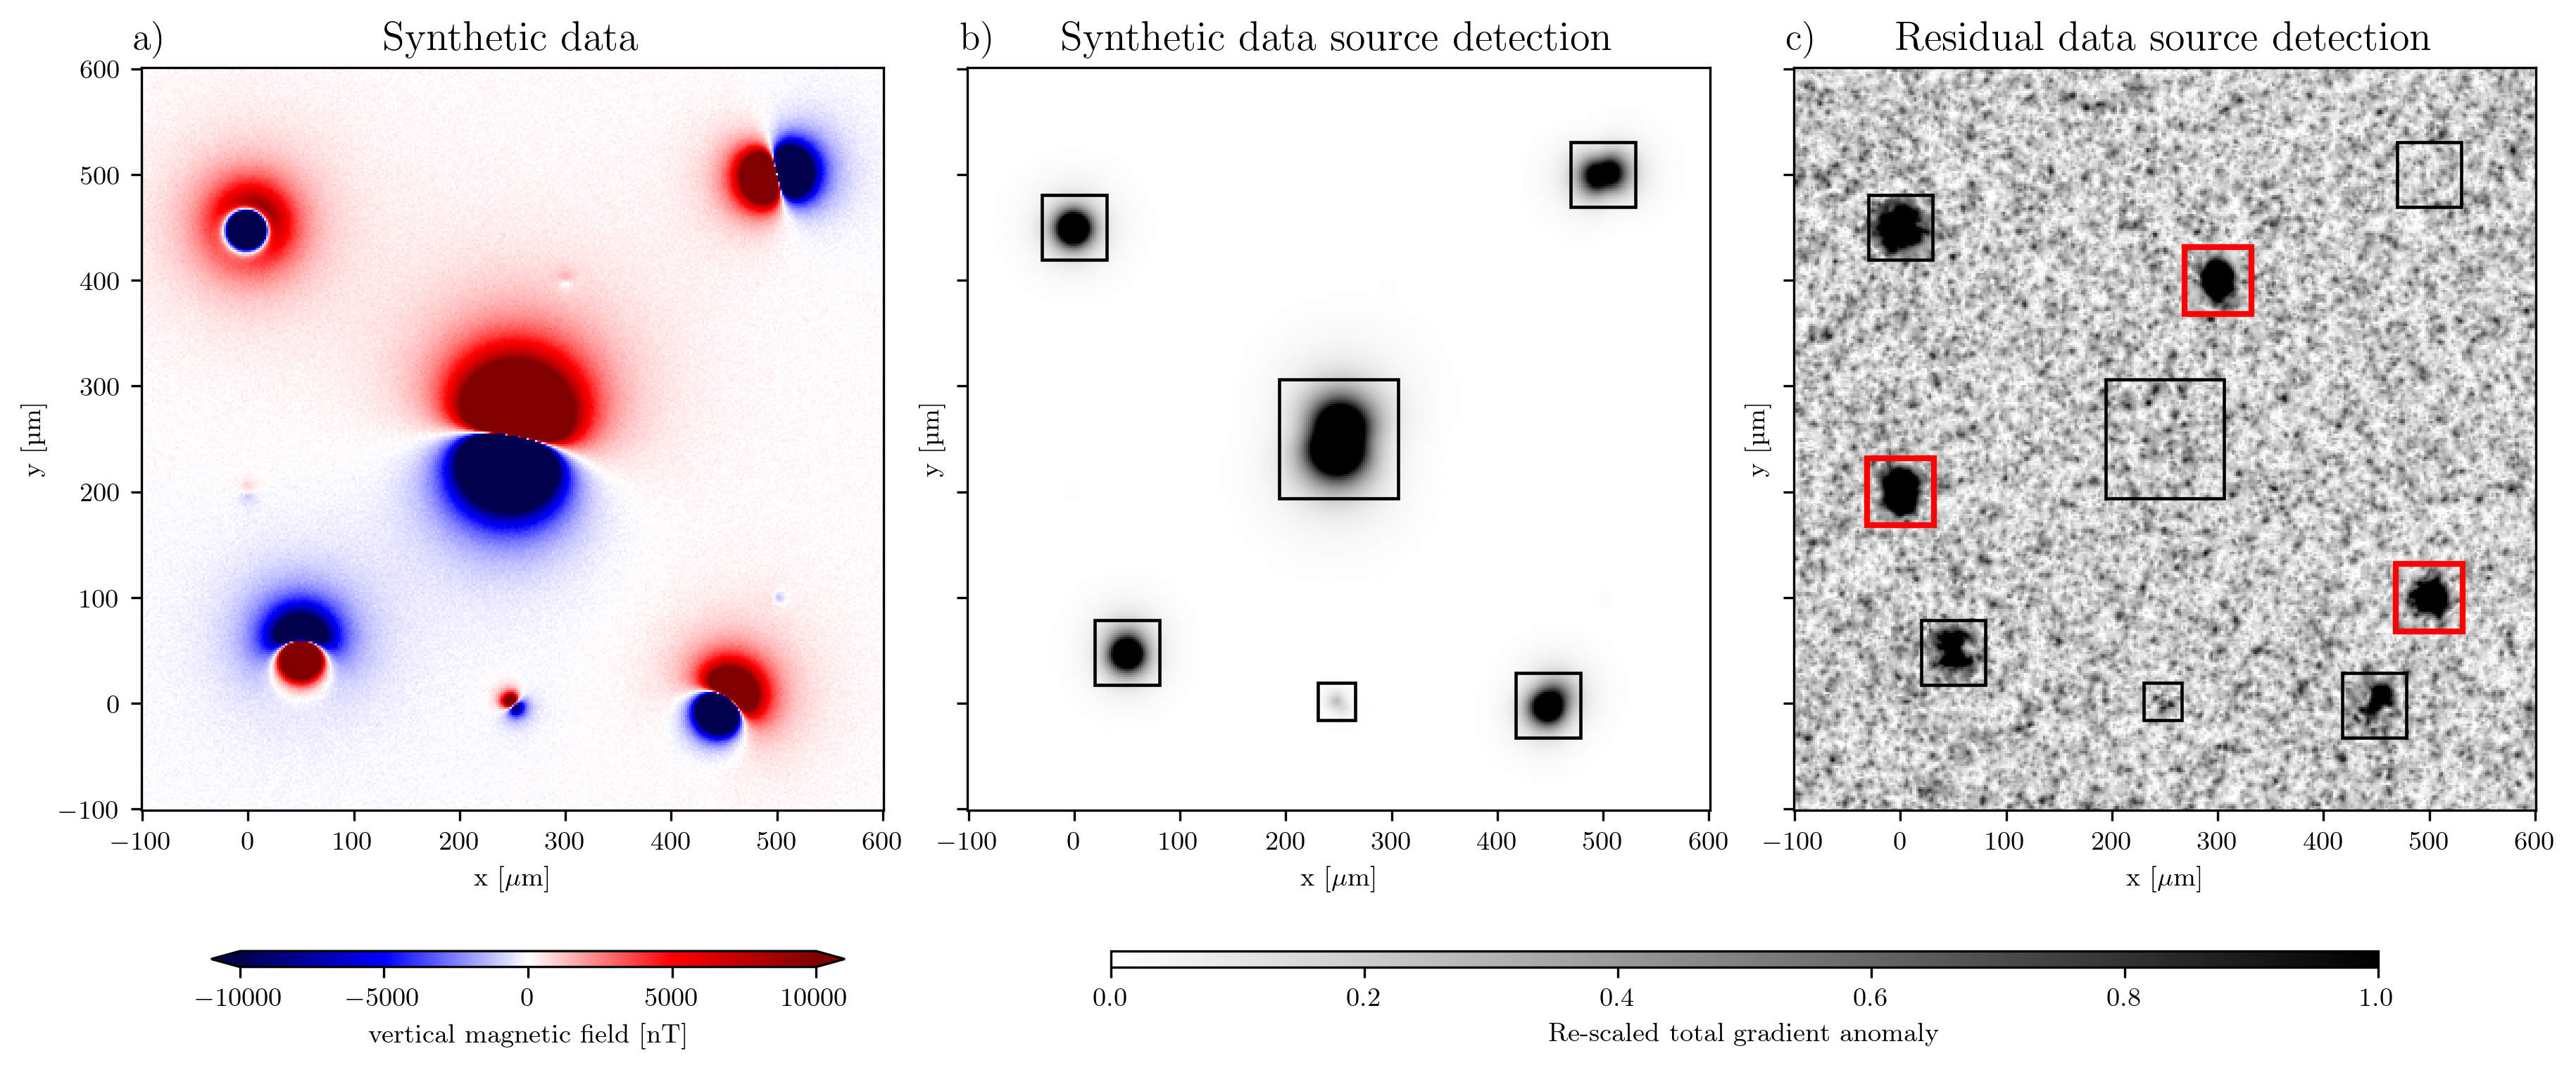
\includegraphics[width=1\linewidth]{paper/figures/re-detection-methodology.png}
      \caption{Workflow to perform the source detection on the residual anomaly. a) Synthetic sample featuring a wide range of magnetic moment intensity. b) The Blob detection algorithm result uses the total gradient obtained with the vertical component of the magnetic field. c) Blob detection algorithm result using the total gradient of the residual anomaly.}
      \label{method-redetection}
    \end{figure}


%%%%%%%%%%%%%%%%%%%%%%%%%%%%%%%%%%%%%%%%%%%%%%%%%%%%%%%%%%%%%%%%%%%%%%%%%%%%%
\subsection{Criteria for Determining Magnetization Direction}

The selection of vectors for summation followed a rigorous three-step methodology to ensure the robustness and reliability of the results.

\subsubsection{Goodness-of-Fit Assessment}

The first step consisted of evaluating the goodness-of-fit by computing the coefficient of determination ($R^2$). This was done by comparing the real data with the residuals obtained from the developed model:

\begin{equation}
    R^2 = 1 - \frac{\sum_{i} (y_i - \hat{y}_i)^2}{\sum_{i} (y_i - \bar{y})^2},
\end{equation}

where $y_i$ represents the observed data, $\hat{y}_i$ denotes the modeled values, and $\bar{y}$ is the mean of the observed data. A threshold of $R^2 \geq 0.90$ was empirically chosen, ensuring that at least 90\% of the data variance was explained by a dipolar model. This value provided a balanced trade-off between a stringent cutoff and the retention of a statistically significant dataset.

\subsubsection{Outlier Removal}

The second step involved the removal of outliers based on the logarithmic distribution of the magnetic moments ($\log_{10} M$). The magnitude of the magnetic moment was computed using the Euclidean norm:

\begin{equation}
    M = \| \mathbf{m} \| = \sqrt{m_x^2 + m_y^2 + m_z^2},
\end{equation}

where $m_x$, $m_y$, and $m_z$ are the Cartesian components of the magnetic moment. Outliers were identified using the interquartile range (IQR) method, following the principles of a boxplot:

\begin{equation}
    \text{Lower Bound} = Q_1 - 1.5 \times \text{IQR}, \quad \text{Upper Bound} = Q_3 + 1.5 \times \text{IQR},
\end{equation}

where $Q_1$ and $Q_3$ are the first and third quartiles, respectively, and $\text{IQR} = Q_3 - Q_1$.

\subsubsection{Jackknife Resampling}

The final step involved the application of the jackknife resampling technique to enhance the reliability of the vector distribution. To achieve statistical robustness, 50 iterations of the jackknife technique were performed. In each iteration, 20\% of the vectors were randomly removed. The final selected distribution was obtained by computing the median across all iterations:

\begin{equation}
    M_{\text{final}} = \text{median} \{ M_1, M_2, \dots, M_{50} \}.
\end{equation}

This approach ensured that the selected vectors were representative and minimally influenced by outliers or stochastic variations in the dataset, while still maintaining a sufficient number of data points for statistical accuracy.

%%%%%%%%%%%%%%%%%%%%%%%%%%%%%%%%%%%%%%%%%%%%%%%%%%%%%%%%%%%%%%%%%%%%%%
\section{Numerical Simulations}

In this section, we evaluate the effectiveness of the interfering sources method, in comparison with the method proposed by \citet{Souza-Junior2024}, by applying it to two synthetic datasets. The tests are structured as follows:  


\begin{enumerate}
    \item \textbf{Evaluating Overlapping Signal Detection:}
        This test simulates a single map containing both strong and weak sources to evaluate the method's ability to discern and accurately locate the weaker sources despite interference from the stronger ones.
    \item \textbf{Assessing Performance with Variable Particle Density:}
        This test introduces a more complex scenario by simulating a specific magnetization direction for the magnetic sources. Additionally, three different particle density scenarios are modeled to test whether the method can reliably recover the magnetization direction across all cases.
\end{enumerate}

\subsection{Evaluating Overlapping Signal Detection}

The first model scenario consists of several dipole sources with varying moment magnitudes, inclinations, and declinations, organized into three distinct groups. The first group contains 150 dipoles with random orientations and moment magnitudes an order of magnitude larger than those in the second group. The second group comprises 50 dipoles with a stable orientation: an inclination of \(\ang{35}\) (\(\pm \ang{5}\)), a declination of \(\ang{340}\) (\(\pm \ang{5}\)), and dipole moment magnitudes centered at \(1.0 \times 10^{-16} Am^2\). Additionally, a third group includes 9 sporadic, deeper, and strongly magnetized sources with random orientations and significantly higher dipole moments of \(1.0 \times 10^{-11} Am^2\). Which totals 209 magnetic particles.

To evaluate the methodologies, we simulate these magnetic sources randomly distributed within a synthetic thin section measuring \(\qty{2000}{\micro\meter} \times \qty{2000}{\micro\meter}\). The synthetic vertical magnetic field data (\(b_z\)) are generated on a regular grid with \(\qty{2}{\micro\meter}\) spacing and a sensor sample distance of \(\qty{5}{\micro\meter}\), without any external applied field. Thus, the magnetic anomaly is solely caused by their dipole moment. High-frequency pseudo-random noise with a zero mean and a standard deviation of \(\qty{50}{\nano\tesla}\) is added for a realistic approximation of a QDM measurement \citep{Glenn2017}. The modeled sources were positioned at depths ranging from 1 to \(\qty{20}{\micro\meter}\). To further emulate actual acquisition conditions, a positive baseline shift of \(\qty{2000}{\nano\tesla}\) is applied to the magnetic field data. This setup tests the algorithm's robustness and accuracy when handling systematically shifted and noise-corrupted magnetic field measurements, as commonly observed in magnetic microscopy experiments.

The synthetic data inversion was resolved using both the standard method \citep{Souza-Junior2024} and the proposed interfering sources methodology. A summary comparison of the classic Euler method and the iterative approach showed significant results in analyzing the synthetic data. The iterative Euler deconvolution method notably enhanced source detectability, with newly identified windows highlighted (green squares, Figure \ref{euler2}a). Figure \ref{euler2}b displays the 114 sources initially detected from the 209 modeled. Meanwhile, Figure \ref{euler2}c indicates that the iterative Euler method retrieved 165 sources. Initially, it may appear that the iterative method underperforms compared to the standard in terms of 3D source location precision; however, most previously identified sources demonstrate reduced position misfit (barring sporadic deeper ones). The larger misfits in Figure \ref{euler2}c are linked to the newly identified grains, as their smaller dipole moment results in greater error in the Euler estimation. This increase in accuracy is crucial, especially in scenarios where stronger magnetic sources can distort the magnetic field anomaly of weaker sources. Although this new methodology can markedly increase the accuracy in the estimated position for virtually all sources, the biggest errors are still related to clustered sources. Also in both cases, the Euler deconvolution seems unaffected by the presence of a shift in the magnetic field.


\begin{figure}[tb!]
  \centering
  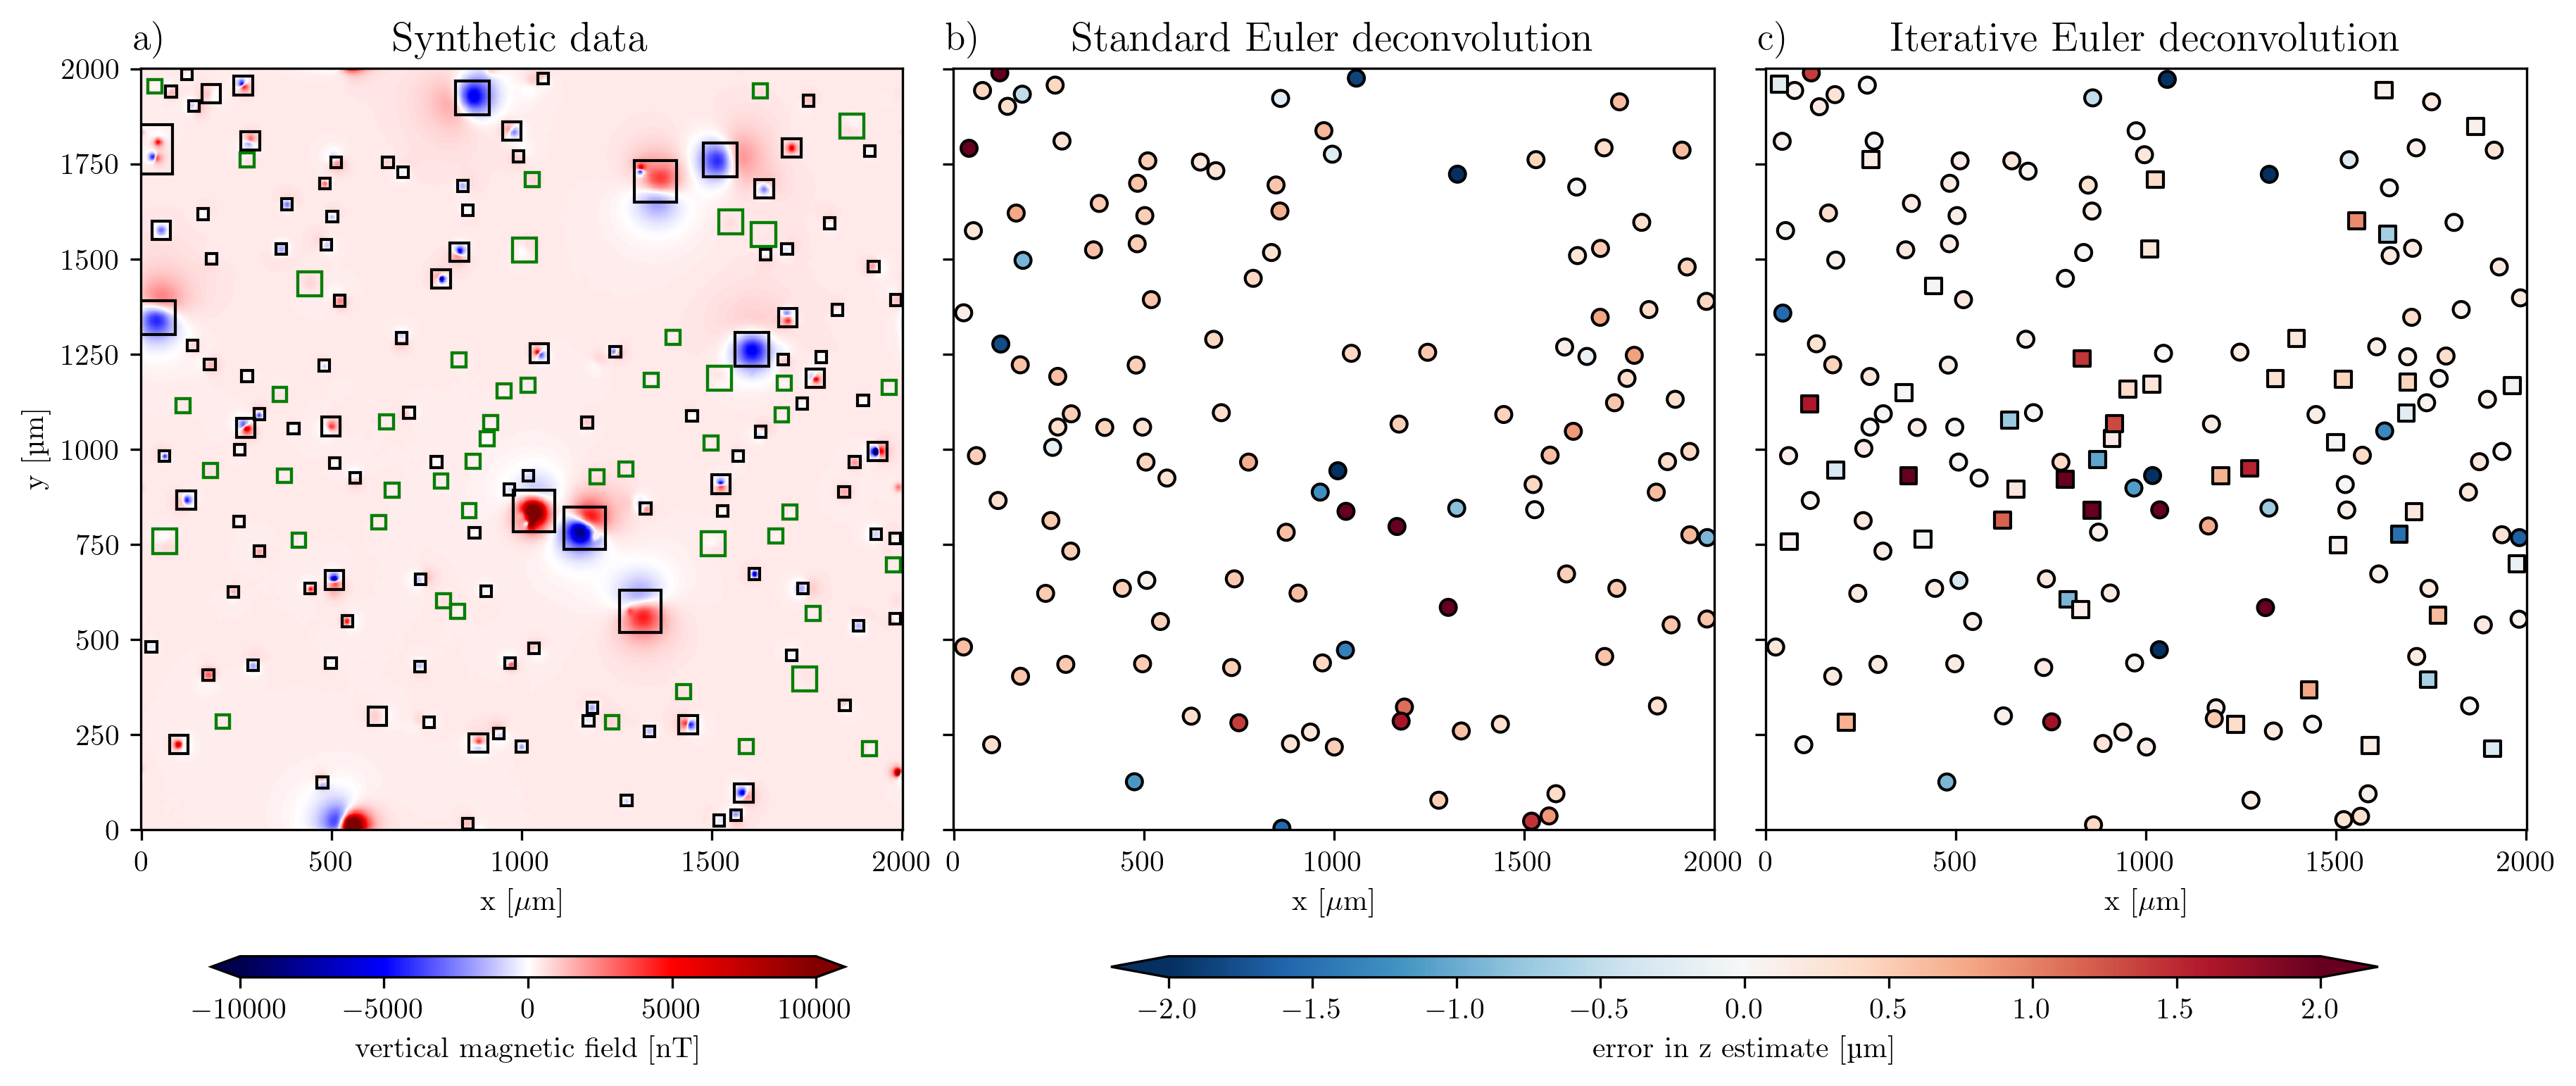
\includegraphics[width=1\linewidth]{paper/figures/euler-comparion-synthetic.png}
  \caption{Complex synthetic sample position estimation. (a) Detection window data of each magnetic source (black squares). These data windows were used in the 3D position estimation of the magnetic sources (colored circles) for the standard (b) and iterative (c) methodologies. }
  \label{euler2}
\end{figure}

These iterative Euler estimated positions were used for the magnetic inversion due to their better results except for the standard method results, which were kept unchanged from the results presented by \citet{Souza-Junior2024}. Figure~\ref{inversion2} summarizes the comparison concerning the angular misfit, the magnetic moment misfit, and the r-squared score, respectively, for the standard (Figures~\ref{inversion2}a-c), and iterative interfering sources (Figures~\ref{inversion2}d-f). Overall, as predicted, the interfering source method outperformed the standard one in all three measured parameters. Nevertheless, the proposed method is fully capable of dealing with tightly clustered sources, especially for the magnetic moment misfit. This observation might have its cause inherited rooted in the limitations of the Euler deconvolution, even after all the improvements of the iterative Euler deconvolution (Figures~\ref{euler2}c), which trigger the ambiguity between the source's depth and its magnetic intensity. This example shows that the proposed methodology can be applied to magnetic microscopy, yielding better results than the original method.


\begin{figure}[tb!]
  \centering
  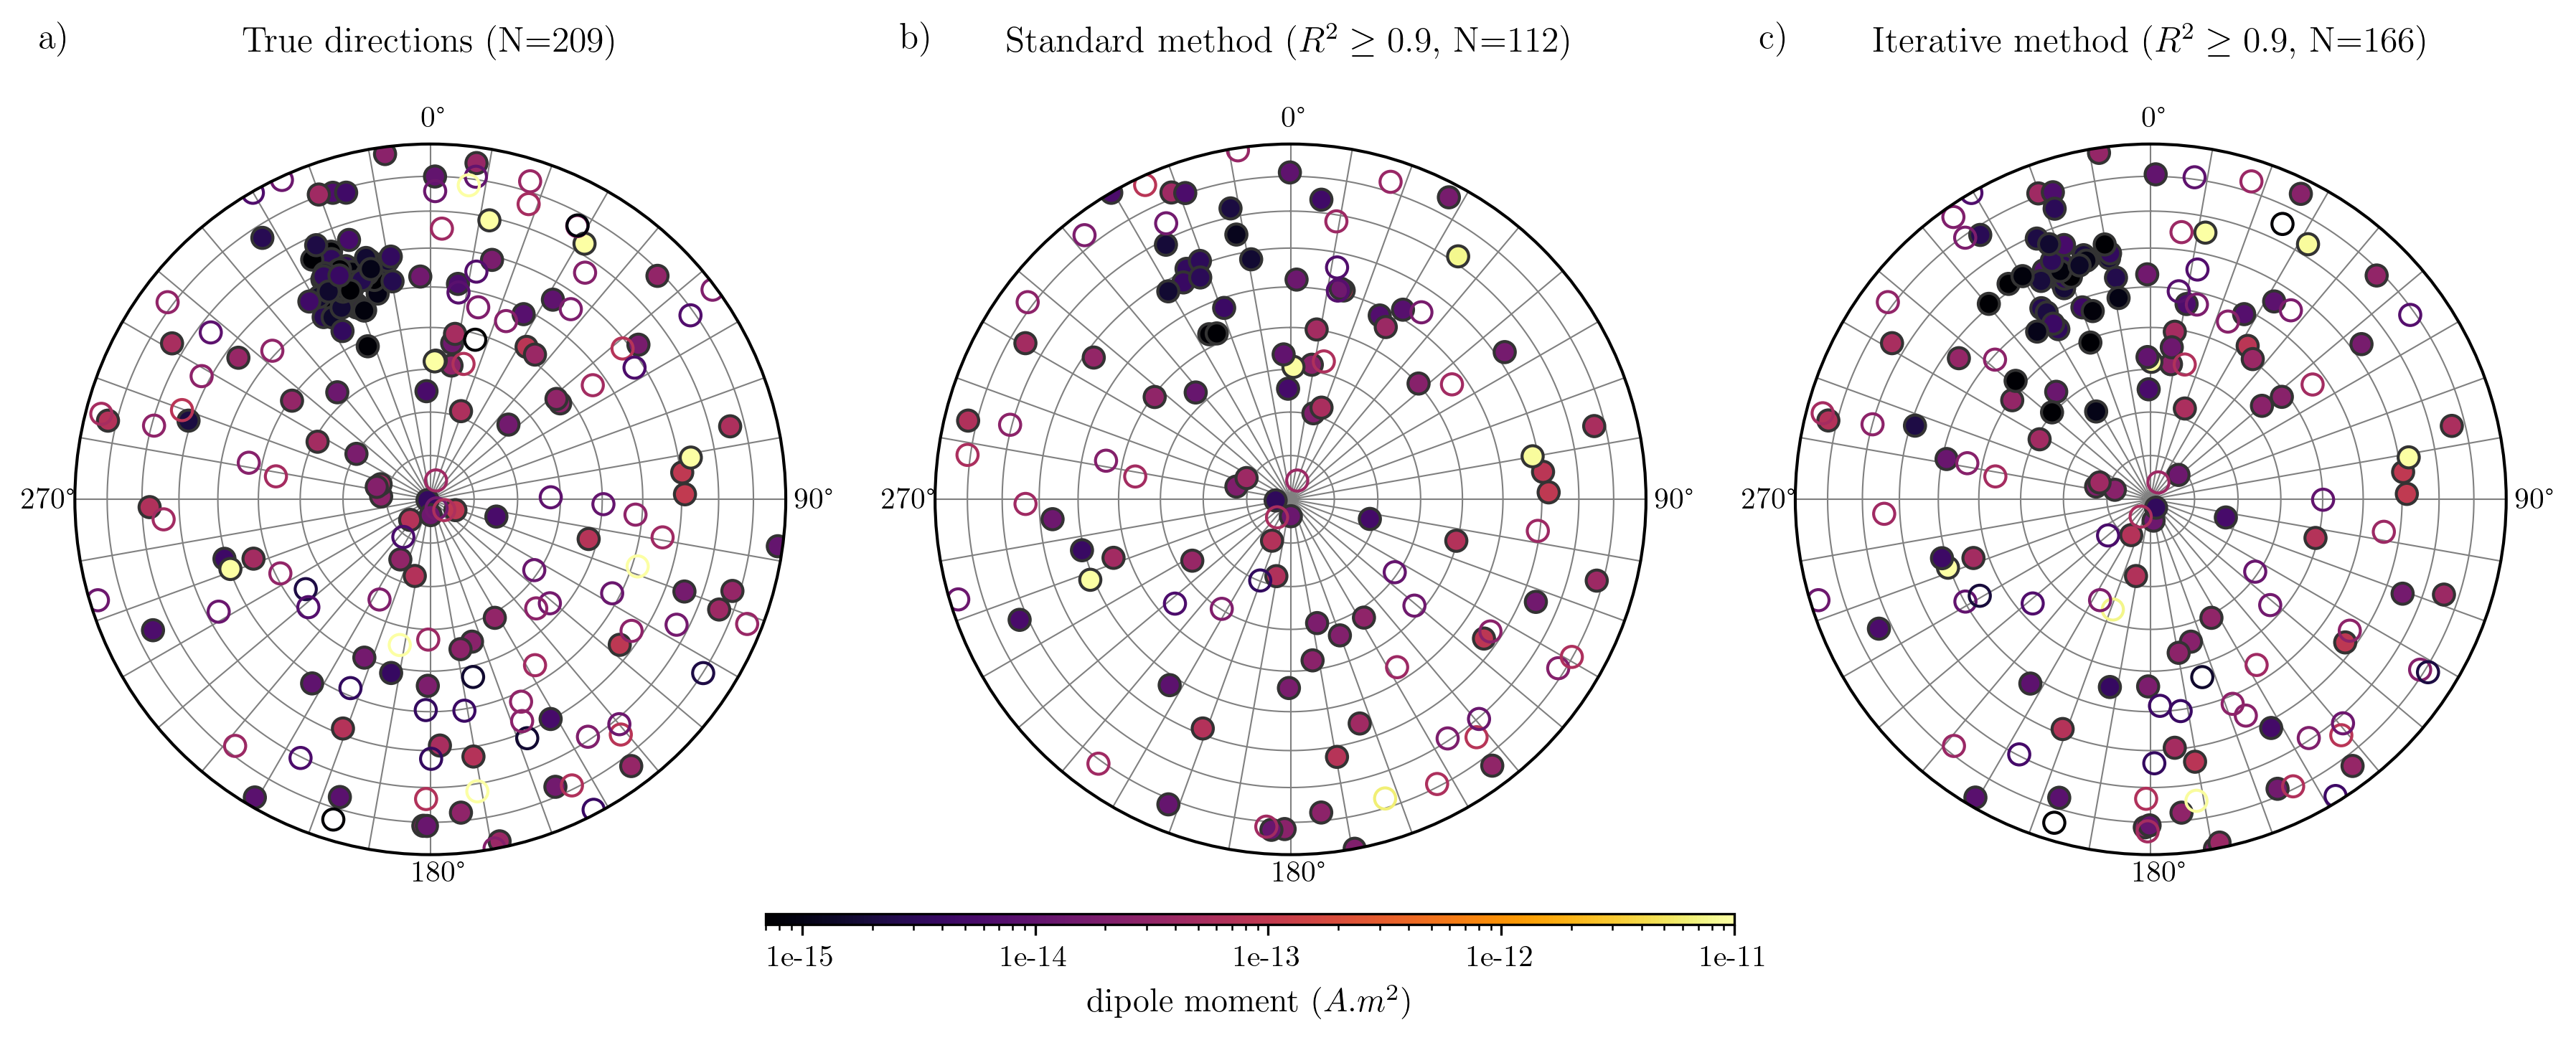
\includegraphics[width=1\linewidth]{paper/figures/synthetic-data-stereograms-comparison.png}
  \caption{Validation of the inversion results/parameters, for each particle, was obtained by computing the real and recovered differences using magnetic direction misfit, misfit of magnetic moment intensity, and the R² score from the model fitting. These parameter were calculated for the standard (a, b, and c, respectively) and iterative (d, e, and f, respectively) methodologies.}
  \label{inversion2}
\end{figure}



\subsection{Assessing Performance with Variable Particle Density}

To assess the impact of particle density on the simulated results, three different grain concentrations were considered, with \(N=500\), \(N=1000\), and \(N=2500\), corresponding to grain densities of approximately \(9000\), \(18000\), and \(45000\,\mathrm{grains/mm^3}\), respectively. These densities were chosen to numerically simulate concentrations expected in different rock types. Lower densities are typical of rocks with scarce magnetic grains, like carbonates, while the highest density approximates rocks with higher particle concentrations, such as basalts.

The directional parameters and magnetic moment intensities distributions were kept constant across all simulations, as the goal was to isolate the effects of increasing particle density. For each simulation, the total \(N\) magnetic dipole sources were created and randomly distributed across a thin section of \qty{2000}{\um} \(\times\) \qty{1400}{\um}. The dipole moments were sampled from a lognormal distribution centered at a mean amplitude of \(1 \times 10^{-14}\,\mathrm{A \cdot m^2}\), with a standard deviation spanning two orders of magnitude. This configuration ensures that most of the distribution is concentrated around the mean, while also allowing for the presence of particles with magnetic moments as strong as \(10^{-11}\,\mathrm{A \cdot m^2}\), simulating larger particles with a greater influence on the magnetic field compared to weaker particles. The modeled sources are also positioned at depths ranging from 1 to \(\qty{20}{\micro\meter}\).

In real ferromagnetic particles, Natural Remanent Magnetization (NRM) varies among particles but is expected to roughly align with the direction of the inducing field. To mirror this variation in our synthetic data, we set the inclination and declination of directional parameters primarily at 30° and 330°, respectively. A 50° dispersion angle introduced variability within spherical statistics, where directional data extends over a unit sphere rather than Cartesian coordinates. This angle indicates a broad spread of directions around the mean, accounting for significant variability in dipole directions, which is crucial for accurately representing the natural diversity of magnetic sources.

The synthetic magnetic field \(b_z\) was computed over a grid with a \qty{2}{\um} spacing, and the measurement plane was set at a constant height of \qty{5}{\um} above the thin section. High-frequency pseudo-random noise, following a Gaussian distribution with zero mean and a standard deviation of \qty{50}{\nano\tesla}, was added to the computed field to mimic realistic measurement conditions. Additionally, a pseudo-random baseline shift ranging from \(-2000\) to \(2000\,\mathrm{nT}\) was introduced to replicate the acquisition process in magnetic microscopy.

The simulations were conducted in a zero external field environment, simulating real acquisitions typically performed in magnetically shielded rooms to eliminate the influence of the Earth's geomagnetic field. The resulting magnetic field data were exported to NetCDF format for further analysis.


\begin{figure}[tb!]
  \centering
  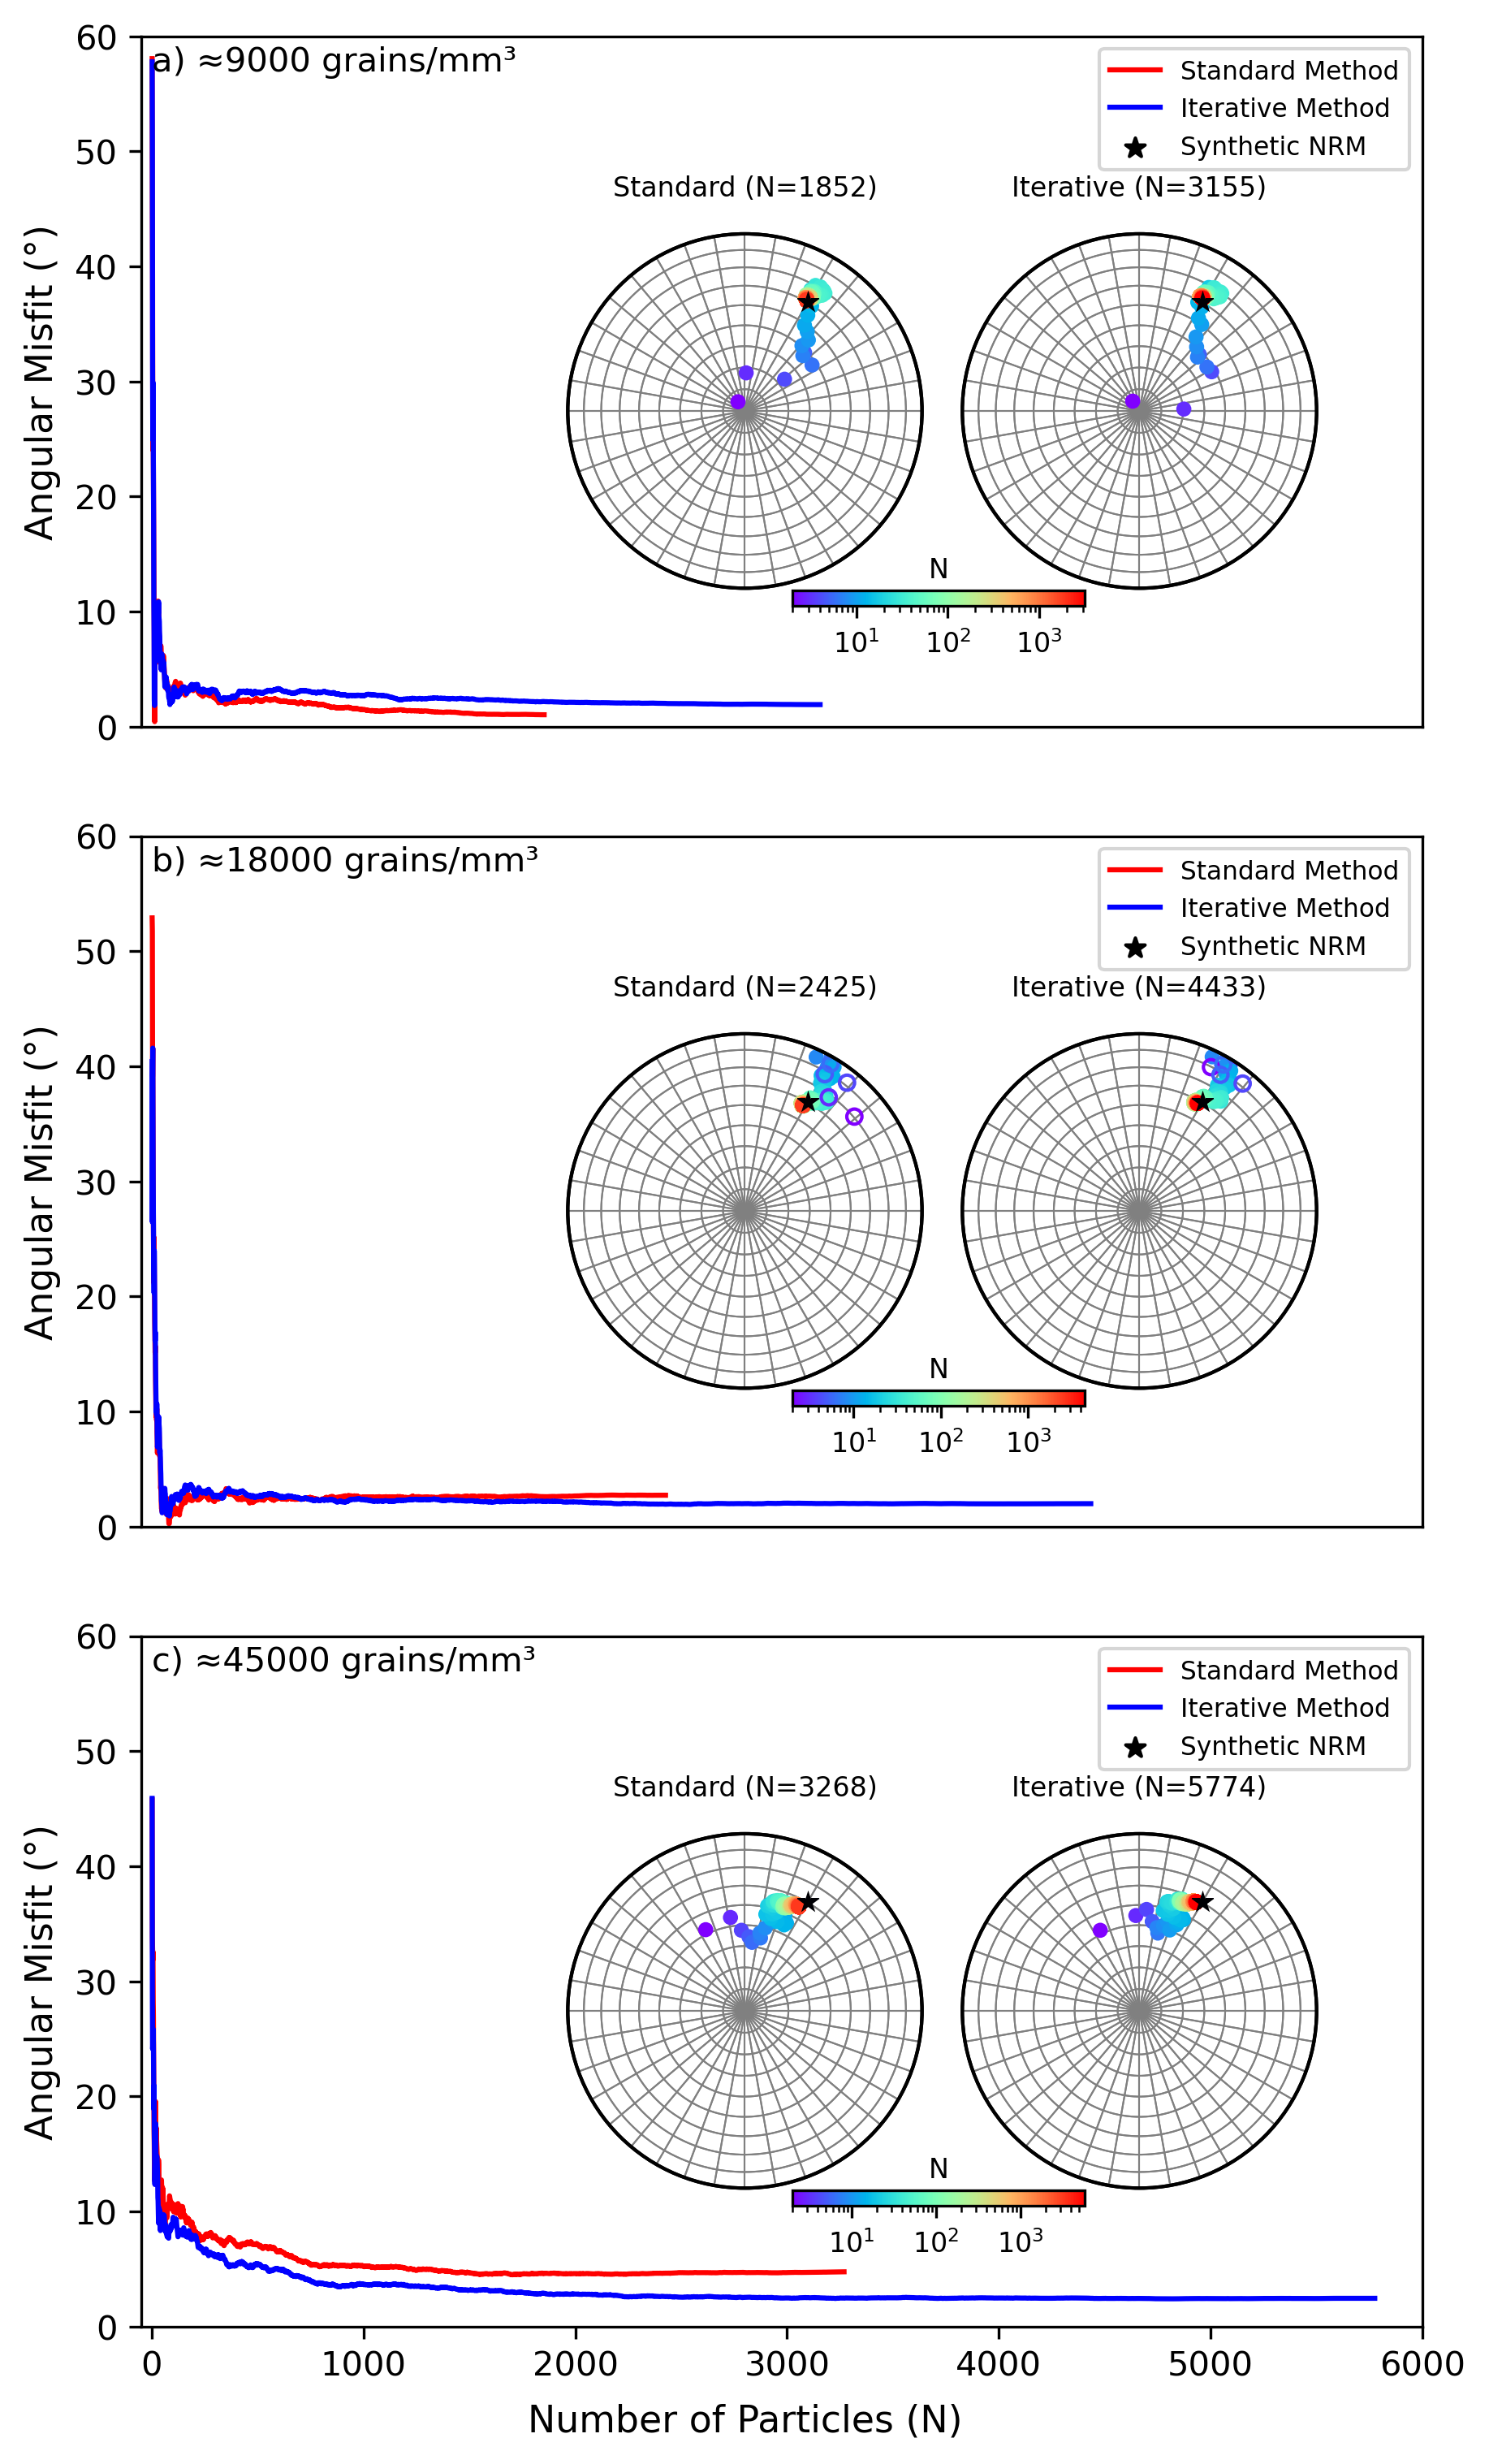
\includegraphics[width=0.7\linewidth]{paper/figures/synthetic-different-densities-stereoplot.png}
  \caption{
blablabla
  }
  \label{synthetic-data-stereograms}
\end{figure}



\section{Real Data Application}

After proving the applicability of the new methodology through the numerical simulations, we can apply it to real sample dataset. To achieve this, we can rely on thermoremanent magnetizations (TRMs) as they represent the most stable means of studying the Earth's geomagnetic field. The magnetic particles \citep[most commonly magnetite,][]{OReilly1984} acquire TRM as they cool below their Curie temperature, with the magnetization direction becoming "locked in" upon reaching the blocking temperature \citep{Dunlop1997}. When grains are sufficiently small and exhibit homogeneous, unidirectional magnetization (single domain, SD), the acquisition and preservation of magnetic signals are physically supported by Néel’s theory \citep{Neel1949, Neel1955}. This allows them to retain remanent magnetization for billions of years, making them excellent recorders of the paleomagnetic field. In addition to SD particles, pseudo-single domain (PSD) particles—characterized by flower and vortex states—are also stable and can preserve magnetization for timescales comparable to the age of the Solar System \citep{Nagy2017, Lascu2018}. Conversely, Néel’s theory does not apply to larger particles (multidomain, MD), which have unstable remanent magnetization \citep[e.g., due to viscous domain reorganization,][]{DeGroot2014}, limiting their capacity to reliably record the geomagnetic field. In this section, we will work with two distinct samples that acquired thermoremanent magnetization (TRM). The natural remanent magnetization (NRM) of the samples was measured using the 2G RAPID Superconducting Rock Magnetometer at the Harvard Paleomagnetics Lab, Department of Earth and Planetary Sciences, Harvard University. As a result, the measurements encompass both the TRM and any viscous components acquired over the years.

\begin{enumerate}
\item \textbf{Evaluation with a Stable Assembly:}
The first test focuses on the analysis of the archaeological ceramic thin-section sample. This sample is characterized by a mid-term density of magnetic particles, with most of them falling into SD and PSD categories. The goal of this test is to assess the method’s performance in real samples where the magnetic carriers are stable, and the influence of unstable domains is minimal. This setting allows for a clear evaluation of the methodology’s sensitivity and accuracy when working with well-defined magnetic signals.

\item \textbf{Evaluation with a Complex Densely Packed Assembly:}
The second test involves the examination of the basaltic rock sample. This sample acquired its TRM during the natural cooling process of lava, leading to a high density of magnetic particles. Unlike the ceramic sample, the basalt is significantly influenced by unstable MD particles, which introduce additional complexity to the magnetic signal. The aim of this test is to verify the method’s effectiveness in identifying and analyzing magnetic sources in challenging conditions, where densely packed magnetic carriers and the presence of unstable remanent magnetization could affect the reliability of the results. This contrast presents a more complex scenario, challenging the methodology to accurately identify and interpret magnetic sources in samples with densely packed and less stable magnetic carriers.
\end{enumerate}


\subsection{Evaluation with a Stable Assembly}

To evaluate the feasibility of magnetic microscopy techniques in detecting and characterizing TRM, we selected a well-preserved fragment of baked clay pavement tile (sample RSLG1) from the archaeological site São Luiz Gonzaga reduction (1657-1687 AD). This fragment was collected by \citet{Poletti2016} and was subsequently used in a paleointensity study, yielding an average intensity of $40.2 \pm 2.4\ \mu\text{T}$ (at 1657–1687 AD). According to the same authors, the magnetic properties of the sample indicate that magnetization is carried by a low-coercivity phase, most likely Ti-poor titanomagnetite in a pseudo-single domain state. This is supported by the IRM acquisition curves saturated at fields up to approximately 0.3 T, narrow hysteresis loops, and maximum NRM demagnetization temperatures around 550°C. FORC diagrams also confirm a predominance of non-interacting single domain to pseudo-single domain grains. These characteristics make the sample an ideal candidate for magnetic microscopy studies aimed at investigating its natural remanent magnetization.

In this study, the vertical component of the magnetic field ($b_z$) was scanned directly from the NRM of the sample using the Quantum Diamond Microscope (QDM) at the Harvard Paleomagnetics Lab (Department of Earth and Planetary Sciences, Harvard University). A total of 20 randomly selected regions were subjected to this scanning procedure to ensure representative coverage of the sample's magnetic properties. The scanned area measured $\qty{1410}{\um} \times \qty{2256}{\um}$ with a grid spacing of \qty{2.35}{\um} ($N = 576 \times 10^{3}$). Data acquisition was conducted at a constant sensor-sample distance of \qty{5}{\um} in a background magnetic field of $< \qty{1}{\micro\tesla}$, provided by the magnetically shielded room. This allowed for high-resolution mapping of the magnetic field distribution.

Both algorithms, the standard and the iterative, were applied, and all magnetic vectors associated with the identified particles were compiled into a database. This dataset was filtered based on the model's coefficient of determination ($R^2$), with only vectors meeting the criterion of $R^2 \geq 0.9$ being retained. This threshold was empirically chosen as it ensures a good fit while not being overly restrictive, thereby maintaining a sufficient number of particles for statistical analysis. The selected vectors were then ordered by intensity and progressively summed. At each step, the cumulative vector was compared with the NRM measured using the 2G RAPID Superconducting Rock Magnetometer.  

The Figure~\ref{ceramic-data-stereograms} illustrates the performance of the standard and iterative algorithms in reconstructing the NRM direction. The left plot shows the angular misfit between the cumulative magnetic vector and the measured NRM as a function of the number of particles ($N$) included in the summation. The standard method (red line) exhibits a higher angular misfit that stabilizes around \ang{55}, while the iterative method (blue line) rapidly reduces the misfit, reaching values close to \ang{10}. The stereographic projections on the right display the directional distribution of the filtered vectors for each method, with color intensity representing the number of particles contributing to each direction. The measured NRM is marked with a star, and the jackknife mean direction is shown as a square.

The lack of significant improvement in the directional accuracy, even with the addition of more particles, may be associated with human-induced errors during the measurement process. Specifically, the sample had to be manually positioned and oriented both in the QDM and in the 2G magnetometer. For the latter, the sample was measured in a vertical orientation and subsequently rotated to align with the reference frame of the thin section used in the QDM analyses. This manual handling and reorientation process could introduce small but cumulative misalignments, contributing to the observed directional discrepancies. 

\begin{figure}[tb!]
  \centering
  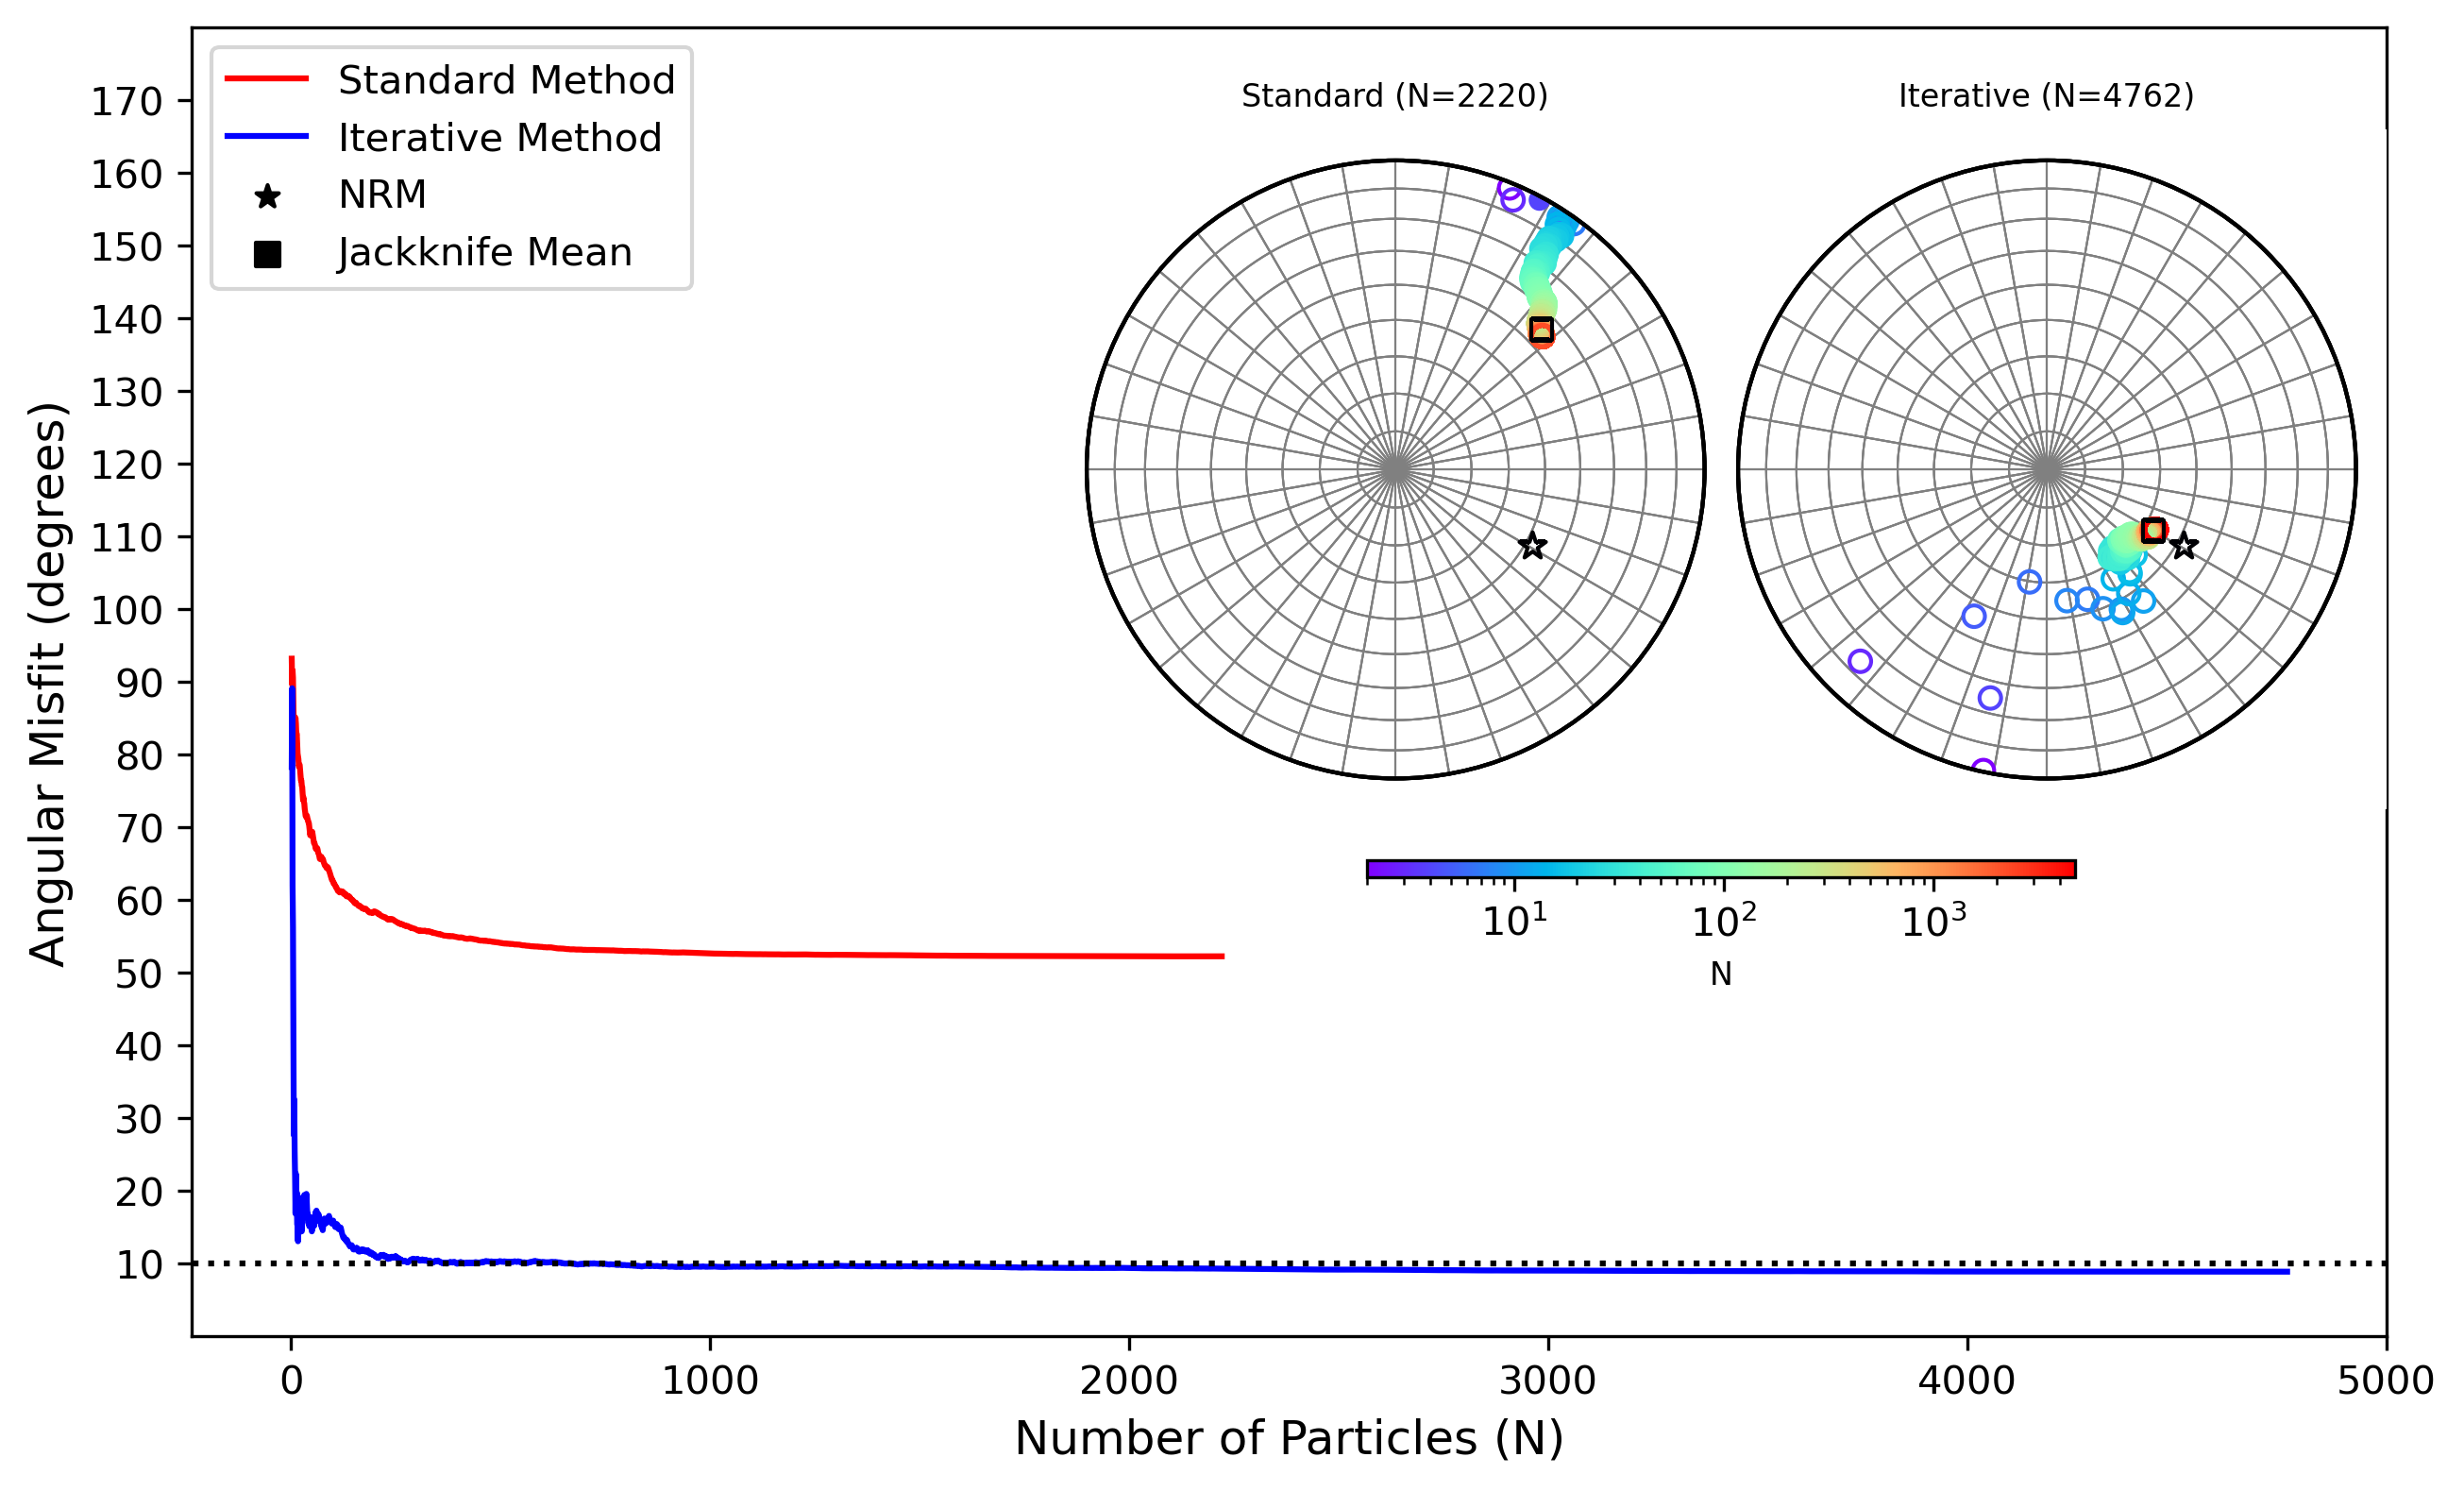
\includegraphics[width=1\linewidth]{paper/figures/ceramic-data-stereoplot.png}
  \caption{
  Comparison of the standard (red) and iterative (blue) algorithms in reconstructing the NRM direction from the ceramic sample. (Left) Angular misfit between the cumulative vector and the measured NRM as a function of the number of particles ($N$). (Right) Stereographic projections of the filtered magnetic vectors ($R^2 \geq 0.9$) for both methods, with the measured NRM (star) and the jackknife mean (square) indicated.The color gradient denotes the logarithmic scale of particle counts, with warmer colors representing higher concentrations.
  }
  \label{ceramic-data-stereograms}
\end{figure}

%%%%%%%%%%%%%%%%%%%%%%%%%%%%%%%%%%%%%%%%%%%%%%%%%%%%%%%%%%%%%%%%%%%%%%%%%%%%%%%
\subsection{Evaluation with a Complex Densely Packed Assembly}

The sample studied belongs to the Caviahue-Copahue volcanic complex (Argentina), specifically a core from the Cola de Zorro Formation (COP01). According to \citet{Moncinhatto2019} this formation presents a preferential alignment of plagioclase crystals, both phenocrysts and smaller crystals in the matrix, exhibiting a trachytic texture. Additionally, it contains a uniform Ti-magnetite population with crystal sizes ranging from 10 to 50 \si{\micro\meter} with low Ti content, given by the Curie temperature around 580~\si{\celsius}. This size distribution is reflected in the high-field experiments, including IRM acquisition curves, hysteresis loops, and FORC diagrams. They reveal saturation at fields around 0.2 \si{T}, coercivities below 10 \si{mT}, and the FORC diagrams are typical of multidomain (MD) grains. Although other samples within the same formation display coercivities between 10 and 20 \si{mT} and FORC diagrams characteristic of magnetite with a PSD behavior, or mixtures of SD and MD grains.

The acquisition of QDM data was essentially the same as the aforementioned experiment with the ceramic tile. The QDM scan was performed to capture the magnetic field distribution at high spatial resolution. The scanning process involved systematically mapping the sample surface, this time ensuring precise alignment and minimizing external interferences. To better compare the results, the same number of randomized mapping spots was performed. The resulting data enabled the calculation of angular misfit as a function of the number of particles, providing insight into the reliability of different analytical methods.

Figure~\ref{basalt-data-stereograms} shows the angular misfit in degrees against the number of particles (N) for both the standard (red line) and iterative (blue line) methods. It highlights that the iterative method achieves lower angular misfit values as the number of particles increases, indicating improved accuracy and consistency. The stereographic projections further compare the directional data obtained by both methods. The standard method shows a broader dispersion of vectors, while the iterative method demonstrates a tighter clustering tending to zero with the increased number of particles, reflecting enhanced precision. The black star represents the natural remanent magnetization (NRM) direction, and the black square indicates the jackknife mean, providing reference points for comparison.

\begin{figure}[tb!]
  \centering
  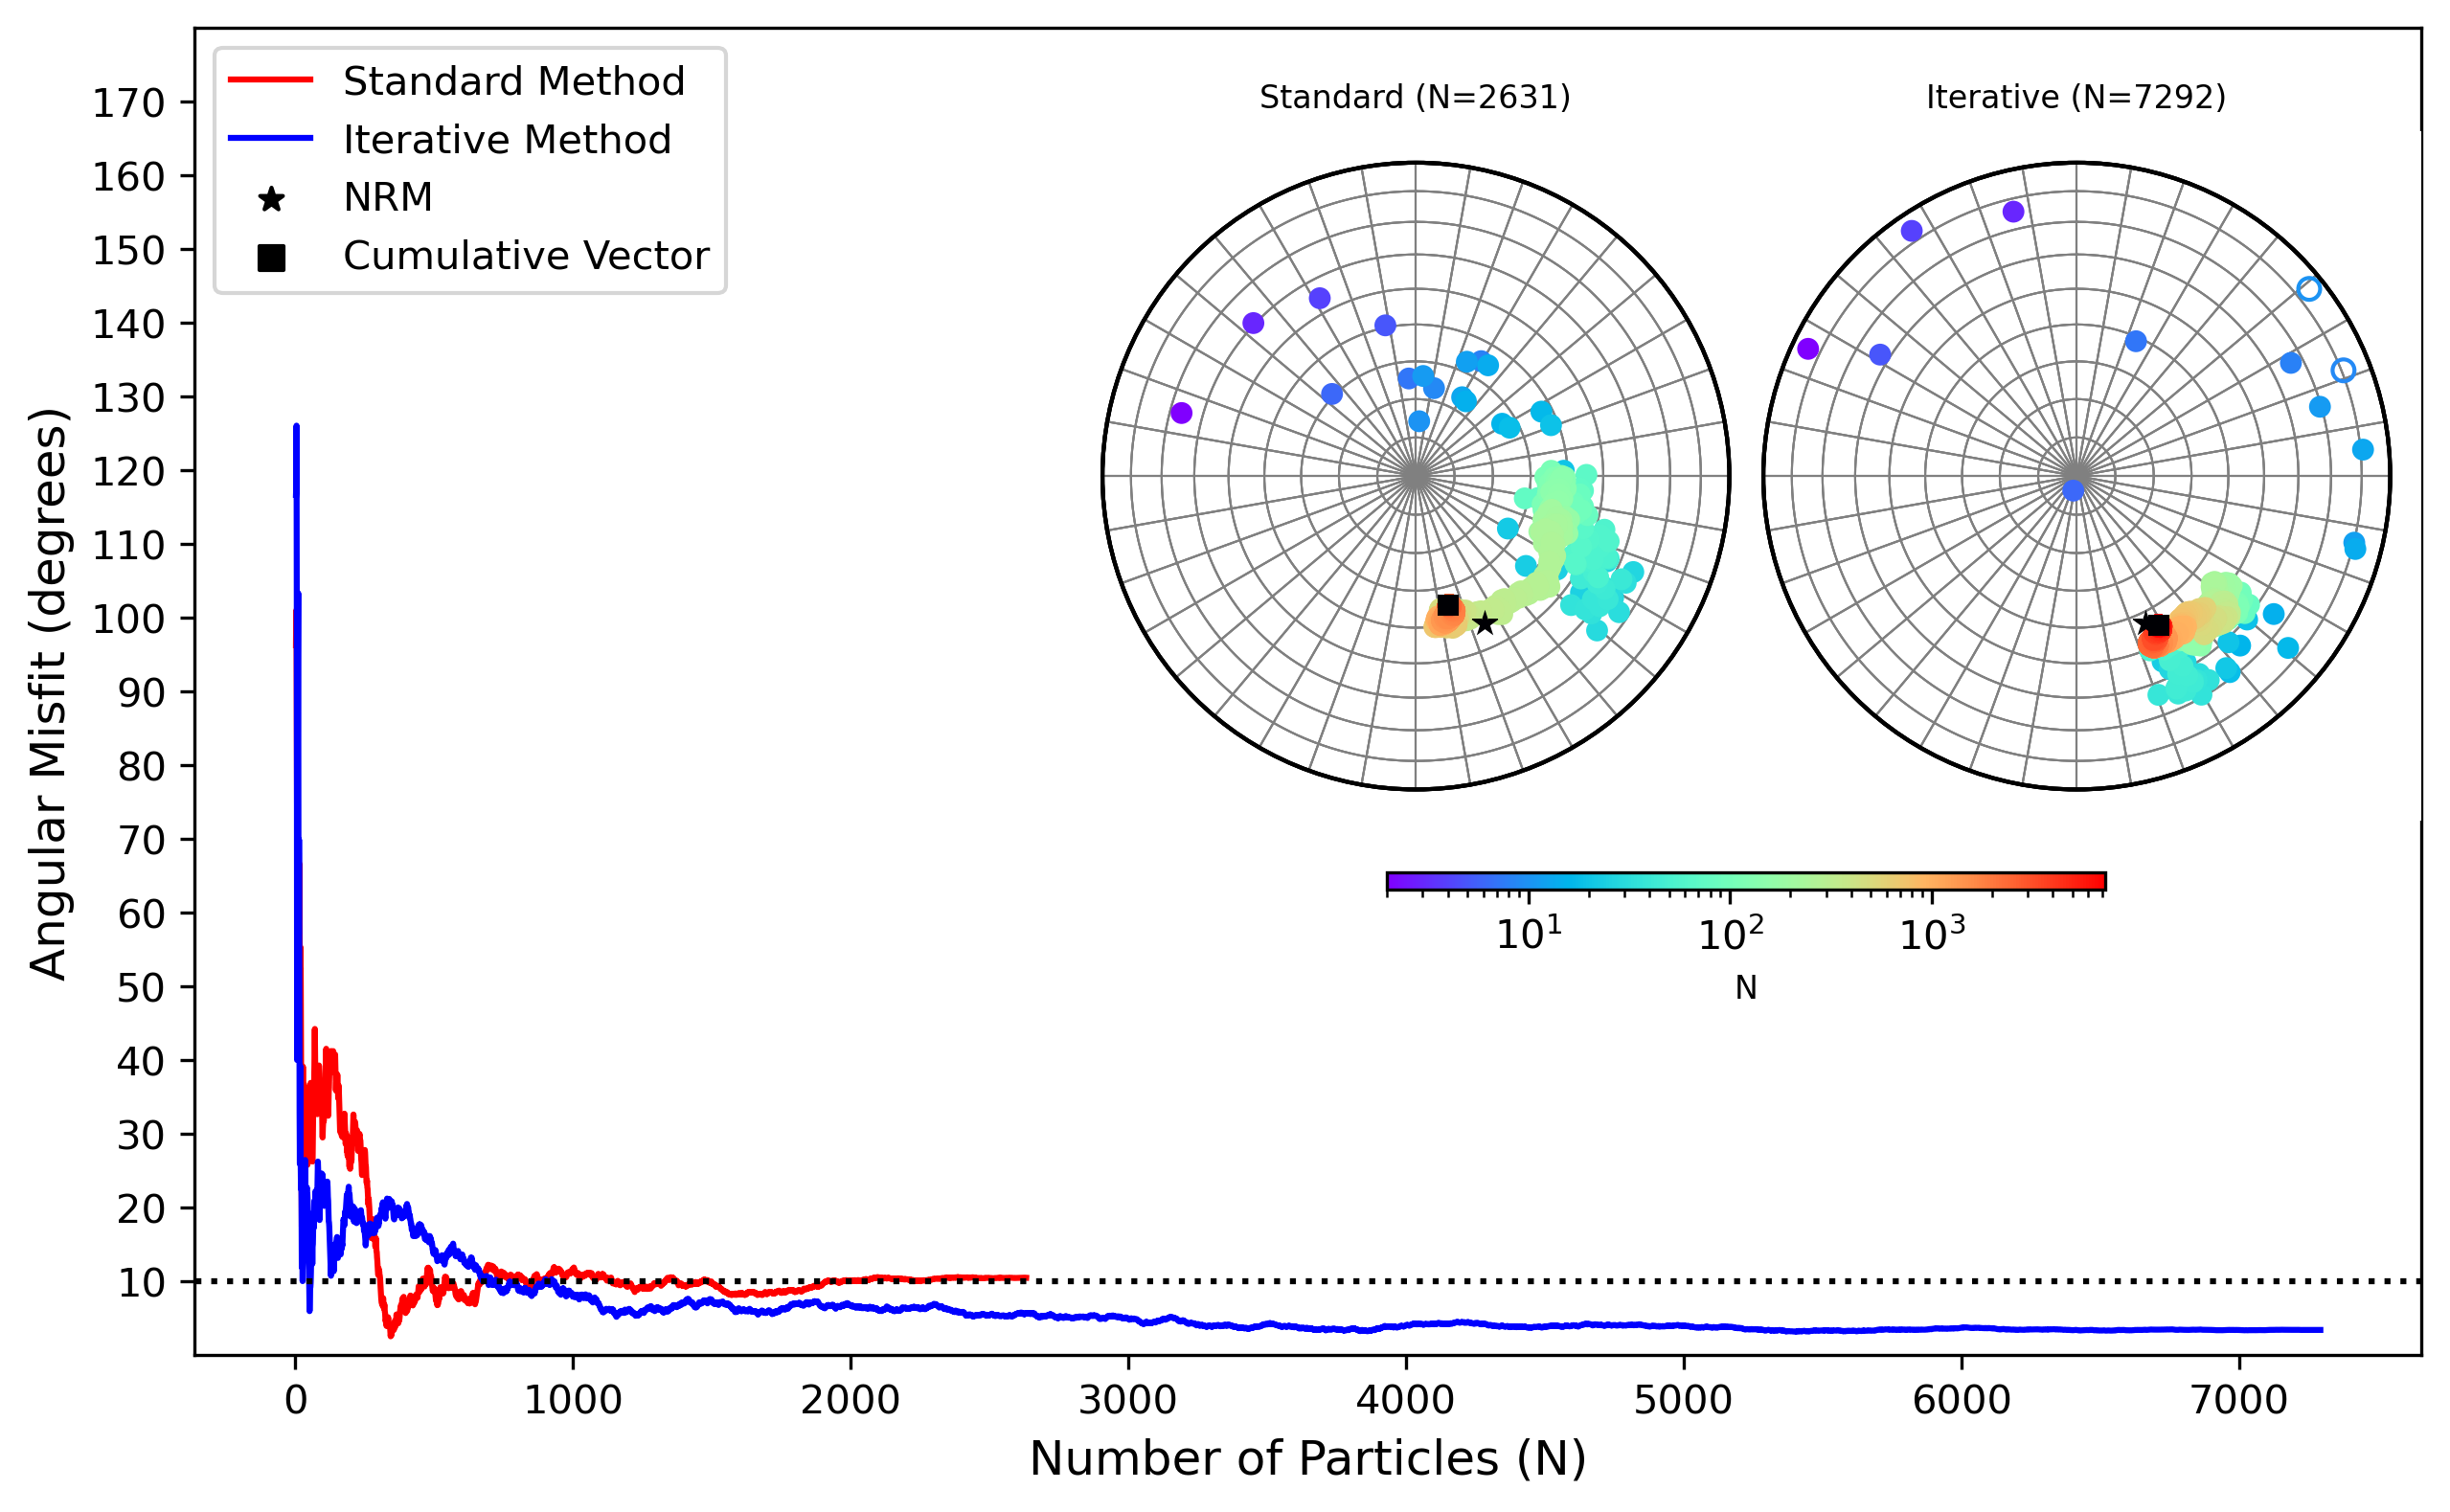
\includegraphics[width=1\linewidth]{paper/figures/basalt-data-stereoplot.png}
  \caption{
  Comparison of the standard (red) and iterative (blue) algorithms in reconstructing the NRM direction from the basalt sample. (Left) Angular misfit between the cumulative vector and the measured NRM as a function of the number of particles ($N$). (Right) Stereographic projections of the filtered magnetic vectors ($R^2 \geq 0.9$) for both methods, with the measured NRM (star) and the jackknife mean (square) indicated. The color gradient denotes the logarithmic scale of particle counts, with warmer colors representing higher concentrations.
  }
  \label{basalt-data-stereograms}
\end{figure}

%%%%%%%%%%%%%%%%%%%%%%%%%%%%%%%%%%%%%%%%%%%%%%%%%%%%%%%%%%%%%%%%%%%%%%%%%%%%%%%
\section{Discussions}

- Comparison and critique about the first paper...
 
The isolated windows approach allows us to separate the area that contains the primary signal of the desired dipole, using the total gradient anomaly, and effectively excluding the region outside the window boundaries, which is less susceptible to variations in the magnetic parameters of this specific source \citep{Souza-Junior2024}. Consequently, we omit this area from the inversion domain. With the application of this technique, it is possible to rapidly determine the 3D position and approximate the dipole moment components of numerous sources in a matter of seconds. This is similar to a method documented by \cite{Weiss2007} by applying a threshold to the long-distance interactions of individual dipoles within the magnetic microscopy data. Through this thresholding, the effect of other dipoles is negated by setting their contributions to zero. However, despite what was stated by \cite{Souza-Junior2023b}, the window segmentation seems to deviate from the core theory of the inversion problem, which mandates that the sampled area must be finite and enclosed within the inversion domain to ensure the uniqueness of results \citep{Baratchart2013, Lima2013}. This insight reveals that the windows approach is effective primarily in contexts with minimal interaction among the sources, or in situations characterized by a sparse presence of magnetic minerals, such as in the case of speleothem samples. Conversely, this approach raises significant concerns in environments with a higher density of sources, such as volcanic rocks, where interactions are more pronounced. This necessitates a thorough reexamination of the existing assumptions, highlighting the need for adaptability in the original methodology to ensure reliability during the paleomagnetic and rock magnetism studies.

Exploring the extent to which the original approach can be utilized successfully is now a critical consideration. To tackle the limitation posed by strong levels of interaction between sources, we incorporated the "interfering sources" methodology, which no longer violates the fundamental theory of the inversion problem. We aim to improve the practicality and precision of the previous approach. Our findings confirm the algorithm's efficacy in mitigating this limitation, especially in situations with prominent source interactions. In such cases, we make a trade-off between accuracy and computational time. However, it is important to note that the interfering sources methodology's efficiency remains relatively constrained when dealing with clustered sources, both for 3D position and dipole moments estimation.

\subsection{Discutir a validacao do methodology (synthetic and real)}




\subsection{discutir com o paper do ualisson}





The application of our methodology to synthetic data reveals promising results, particularly in the accuracy of magnetic direction determination. Nearly all our computed magnetic direction misfits are below 5 degrees (Figure~\ref{inversion2}d), indicating a significant enhancement over the original methodology. Such precision in magnetic direction estimation is a positive outcome for paleomagnetic studies. Moreover, these results satisfy a stringent filtering criterion, with R-squared values greater than or equal to 0.85 for all cases, which means that at least 85\% of the magnetic anomaly is explained by dipolar sources. This high level of model fit demonstrates the robustness of the refined methodology and suggests that it can reliably differentiate between signal and noise, providing a solid foundation for accurate magnetic moment inversion. However, a notable challenge arises when dealing with clusters of closely spaced particles. In these instances, our methodology produces erroneous amplitude results for magnetic moments (Figure~\ref{inversion2}e). We attribute this limitation to the inherited constraints from the Euler deconvolution, which also inaccurately estimates the vertical positioning of particles within clusters, even after the Euler deconvolution enhancement (Figure~\ref{euler2}c). Due to the ambiguity inherent in potential field data, the incorrect vertical positioning likely leads to the erroneous estimation of magnetic moments as the model attempts to compensate for these vertical errors. Therefore, for future paleointensity studies, it is highly recommended to use well-individualized particles to avoid these cluster-related erroneous estimations. Utilizing distinct and separate particles ensures that the magnetic signal is unambiguous, which is critical for accurate paleointensity measurements. This approach reduces the risk of overlapping signals and the potential misinterpretation that can arise from complex magnetic interactions, thus enhancing the reliability of the results obtained.

Afterward, we delve into the application of the enhanced algorithm on actual rock samples, specifically a speleothem, which was initially subjected to two opposing magnetic fields to differentiate the contributions of magnetite and hematite. This separation was observable in the original code (Figure~\ref{real-data-stereograms}a). However, the initial version did not account for some source interference effects, leading to distortions in the results. For stronger particles, this distortion was less pronounced, allowing for a satisfactory fit, as evidenced by an R-squared value greater than 0.85 (Figures~\ref{real-data-stereograms}b). Conversely, smaller or weaker particles, affected by interference from stronger sources or shifts in the measured magnetic field, showed alterations in results. These changes were reflected in the coefficient of determination and failed these particles during the filtering process. With the algorithm's improvement, the effect of these interferences was significantly diminished. Previously, 46 out of 75 particles (approximately 61.33\%) met the selection criteria. With the enhancements in the algorithm, there was a notable improvement in the particle distribution, visible by the readjustment of the smaller particles, which became less dispersed and more concentrated in the directions of the induced magnetic fields (Figures~\ref{real-data-stereograms}c). Furthermore, this improvement is reflected in the increased number of particles meeting the filtering criteria, with 66 particles (88\%) passing the threshold (Figures~\ref{real-data-stereograms}d).

This approach might represent a crucial advancement in the application of magnetic microscopy mapping for paleomagnetic studies. It addresses the critical need to identify tens of thousands of stable fine-grained particles (smaller than \SI{1}{\micro\meter}) and retrieve reliable information from magnetic images, a necessity for imparting statistical robustness to the remanence vector, as highlighted in the findings of \cite{Berndt2016}. While retaining the advantages of being a fast semi-automated approach that does not require any additional measurements. Unfortunately, our methodology also inherits the main problems pointed out by \citet{Souza-Junior2023b}, which are mainly related to the source detectability limitations. In turn, this creates opportunities for further improvements in the algorithm for source detection.





%%%%%%%%%%%%%%%%%%%%%%%%%%%%%%%%%%%%%%%%%%%%%%%%%%%%%%%%%%%%%%%%%%%%%%%%%%%%%%%
\section{Conclusion}
% - Earth and Space Science
% - JGR Machine Learning and Computation

In conclusion, our enhanced algorithm offers significant improvements over its predecessor, particularly in magnetic microscopy mapping for paleomagnetic studies. By refining the isolation of the primary signal and integrating the "interfering sources" algorithm, we have improved the accuracy of 3D position and dipole moment estimations, addressing one of the previous code's limitations. This has led to better particle distribution and increased the number of particles meeting the filtering criteria, demonstrating more reliable magnetic signature detection. Benchmarking against the original method's outcomes substantiates the enhanced reliability and precision of our results, reinforcing the advancement of paleomagnetic data analysis and setting a definitive path for future enhancements.


%%%%%%%%%%%%%%%%%%%%%%%%%%%%%%%%%%%%%%%%%%%%%%%%%%%%%%%%%%%%%%%%%%%%%%%%%%%%%%%
\section{Open research}

% The Python source code used to produce all results and figures presented here, as well as supplemental figures and Jupyter notebooks, are available from \citet{sourcearchive}, which can also be found on \url{https://github.com/\GitHubRepository} under the MIT and CC-BY licenses.
% The QDM magnetic microscopy data are available
% from \citet{janinedata} under the CC-0 license.

% The image re-scaling and blob detection through the Laplacian of Gaussian
% methods were performed with the scikit-image library \citep{VanderWalt2014}.
% We also used matplotlib \citep{Hunter2007} and mplstereonet \citep{mplstereonet}
% for generating figures and stereograms.
% Basic calculations were performed using Numpy \citep{Harris2020} and Scipy
% \citep{2020SciPy-NMeth}.
% Verde \citep{verde2018} was used to generate data grids.
% Upward continuation was performed using Harmonica \citep{harmonica2020}.
% The Choclo library \citep{choclo2022} provided kernel functions used in the
% forward and inverse problems.
% The Numba just-in-time compilation library \citep{lam2015numba} was used to
% speed-up calculations.
% Lastly, the xarray library \citep{hoyer2017xarray} offered a fast and powerful
% tool for working with multi-dimensional datasets allowing an easy way of data
% visualization and extraction with advanced indexing techniques.



%%%%%%%%%%%%%%%%%%%%%%%%%%%%%%%%%%%%%%%%%%%%%%%%%%%%%%%%%%%%%%%%%%%%%%%%%%%%%%%
\section{Acknowledgements}

% We are indebted to the developers and maintainers of the open-source software
% without which this work would not have been possible.
% This research was supported by
% grant 162704/2021-6 from the Conselho Nacional de Desenvolvimento Científico e Tecnológico (CNPq),
% grant 2021/08379-5 from the Fundação de Amparo à Pesquisa do Estado de São Paulo (FAPESP),
% grant PRPI 22.1.09345.01.2 from Universidade de São Paulo,
% and grant IES\textbackslash{}R3\textbackslash{}213141 from the Royal Society.
% The opinions, hypotheses, and conclusions or recommendations expressed in this
% material are the responsibility of the authors and do not necessarily reflect
% the views of FAPESP.


